

\section{Stereo PIV Data Acquisition}

The low speed wind tunnel was outfitted with a stereo particle image 
velocimetry system (PIV) capable of resolving three dimensional velocity vector 
fields within the interrogation plane. Two cameras were mounted with a simple 
frame built from 80$mm$x120$mm$ T-slot extruded aluminum with six sliding 
fastener points on the exterior of the wind tunnel, just outside the test 
section on the left and right sides as shown in figure \ref{fig:pivsetup}. 

\begin{figure}[H]
	\centering
	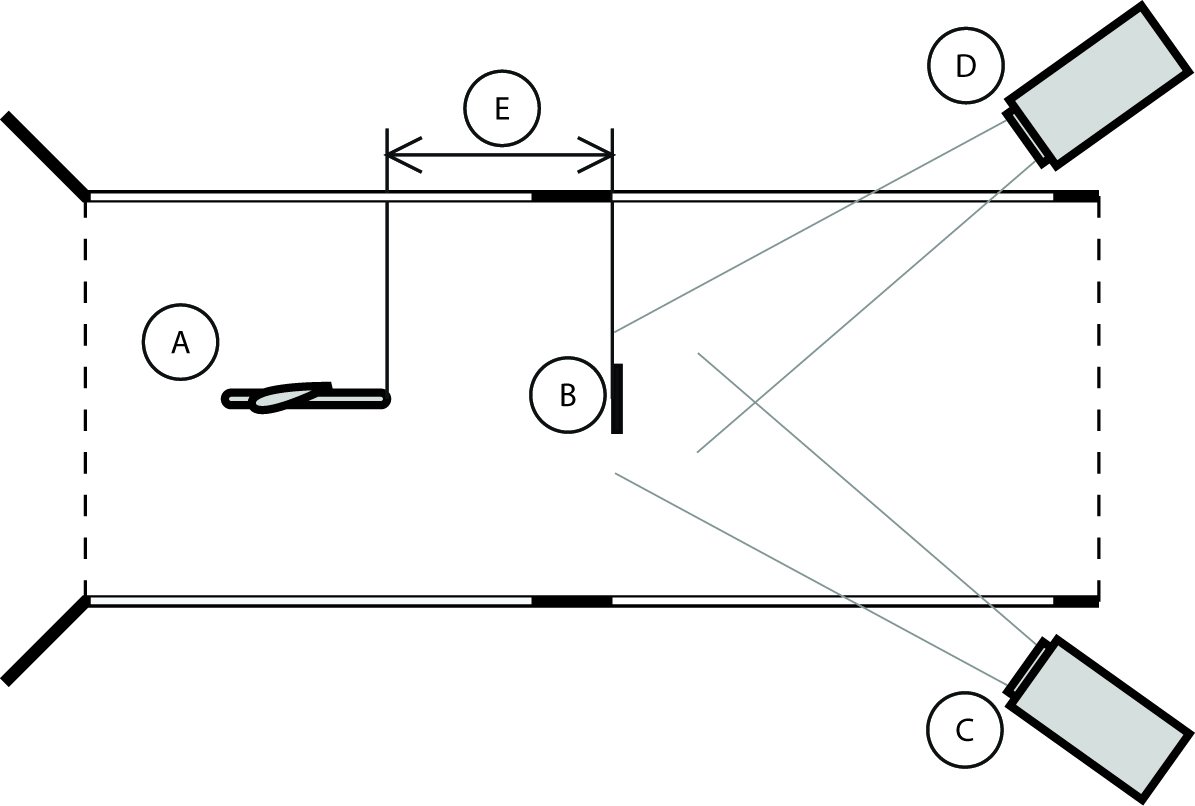
\includegraphics[width=5in]{figs/piv_method/piv_camera_diagram}
	\caption{Top view schematic of PIV camera positions. A-vortex generator, 
	B-PIV 
		calibration target and interrogation plane, C-left camera, D-right 
		camera, E-station distance dimension.}
	\label{fig:pivsetup}
\end{figure}

Each of these cameras was capable of independently resolving a two-dimensional 
velocity field. An Nd:YAG laser was attached to the roof of the wind tunnel, 
just outside of a glass window and pointed downwards to illuminate a cross 
section of the fluid flow perpendicular to the free stream velocity vector as 
shown in Figure \ref{fig:laser_sheet_picture}. In this image, the fluid flow 
has been freshly seeded near the vortex generator and a vortex structure is 
clearly defined with a visible vortex core. In this figure, the bright lines 
mark the edges of the light curtain.


The equipment used for this study was a "TSI Stereo Image Velocimeter System", 
which consists of a pair of TSI PIV 13-8 cameras (Figure 
\ref{fig:camera_picture}), a TSI synchronizer and frame 
grabber specific to the cameras (Figures \ref{fig:synchronizer} and 
\ref{fig:synchronizer2}), a New Wave Dual Mini-YAG Laser (Figure 
\ref{fig:laser}) and Light Guide, a precision 3-D calibration target for stereo 
PIV camera alignment, and a precision laser traverse system. The particle seed 
was generated by an MDG fog generator (Figure \ref{fig:fog_machine}). A 
software package by TSI named INSIGHT was used for data processing (Figure 
\ref{fig:processing_screenshot}).

\begin{figure}[H]
	\centering
	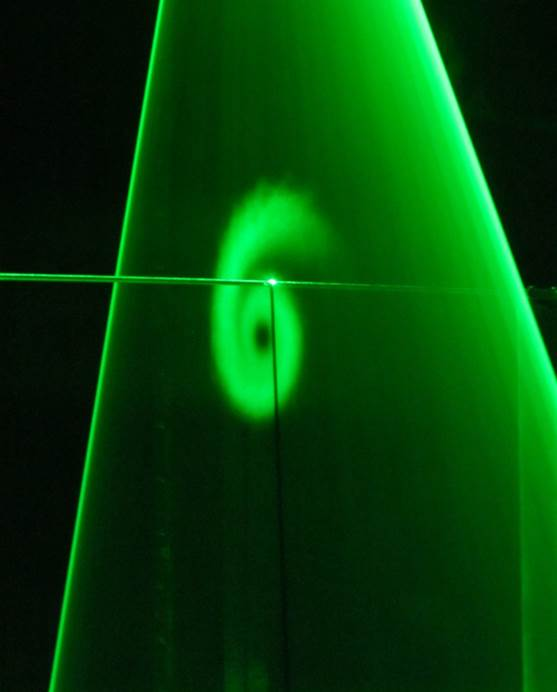
\includegraphics[width=5in]{figs/piv_method/laser_sheet_picture}
	\caption{Picture of a light curtain illuminating a cross section of an 
	axial wake vortex.}
	\label{fig:laser_sheet_picture}
\end{figure}

\begin{figure}[H]
	\centering
	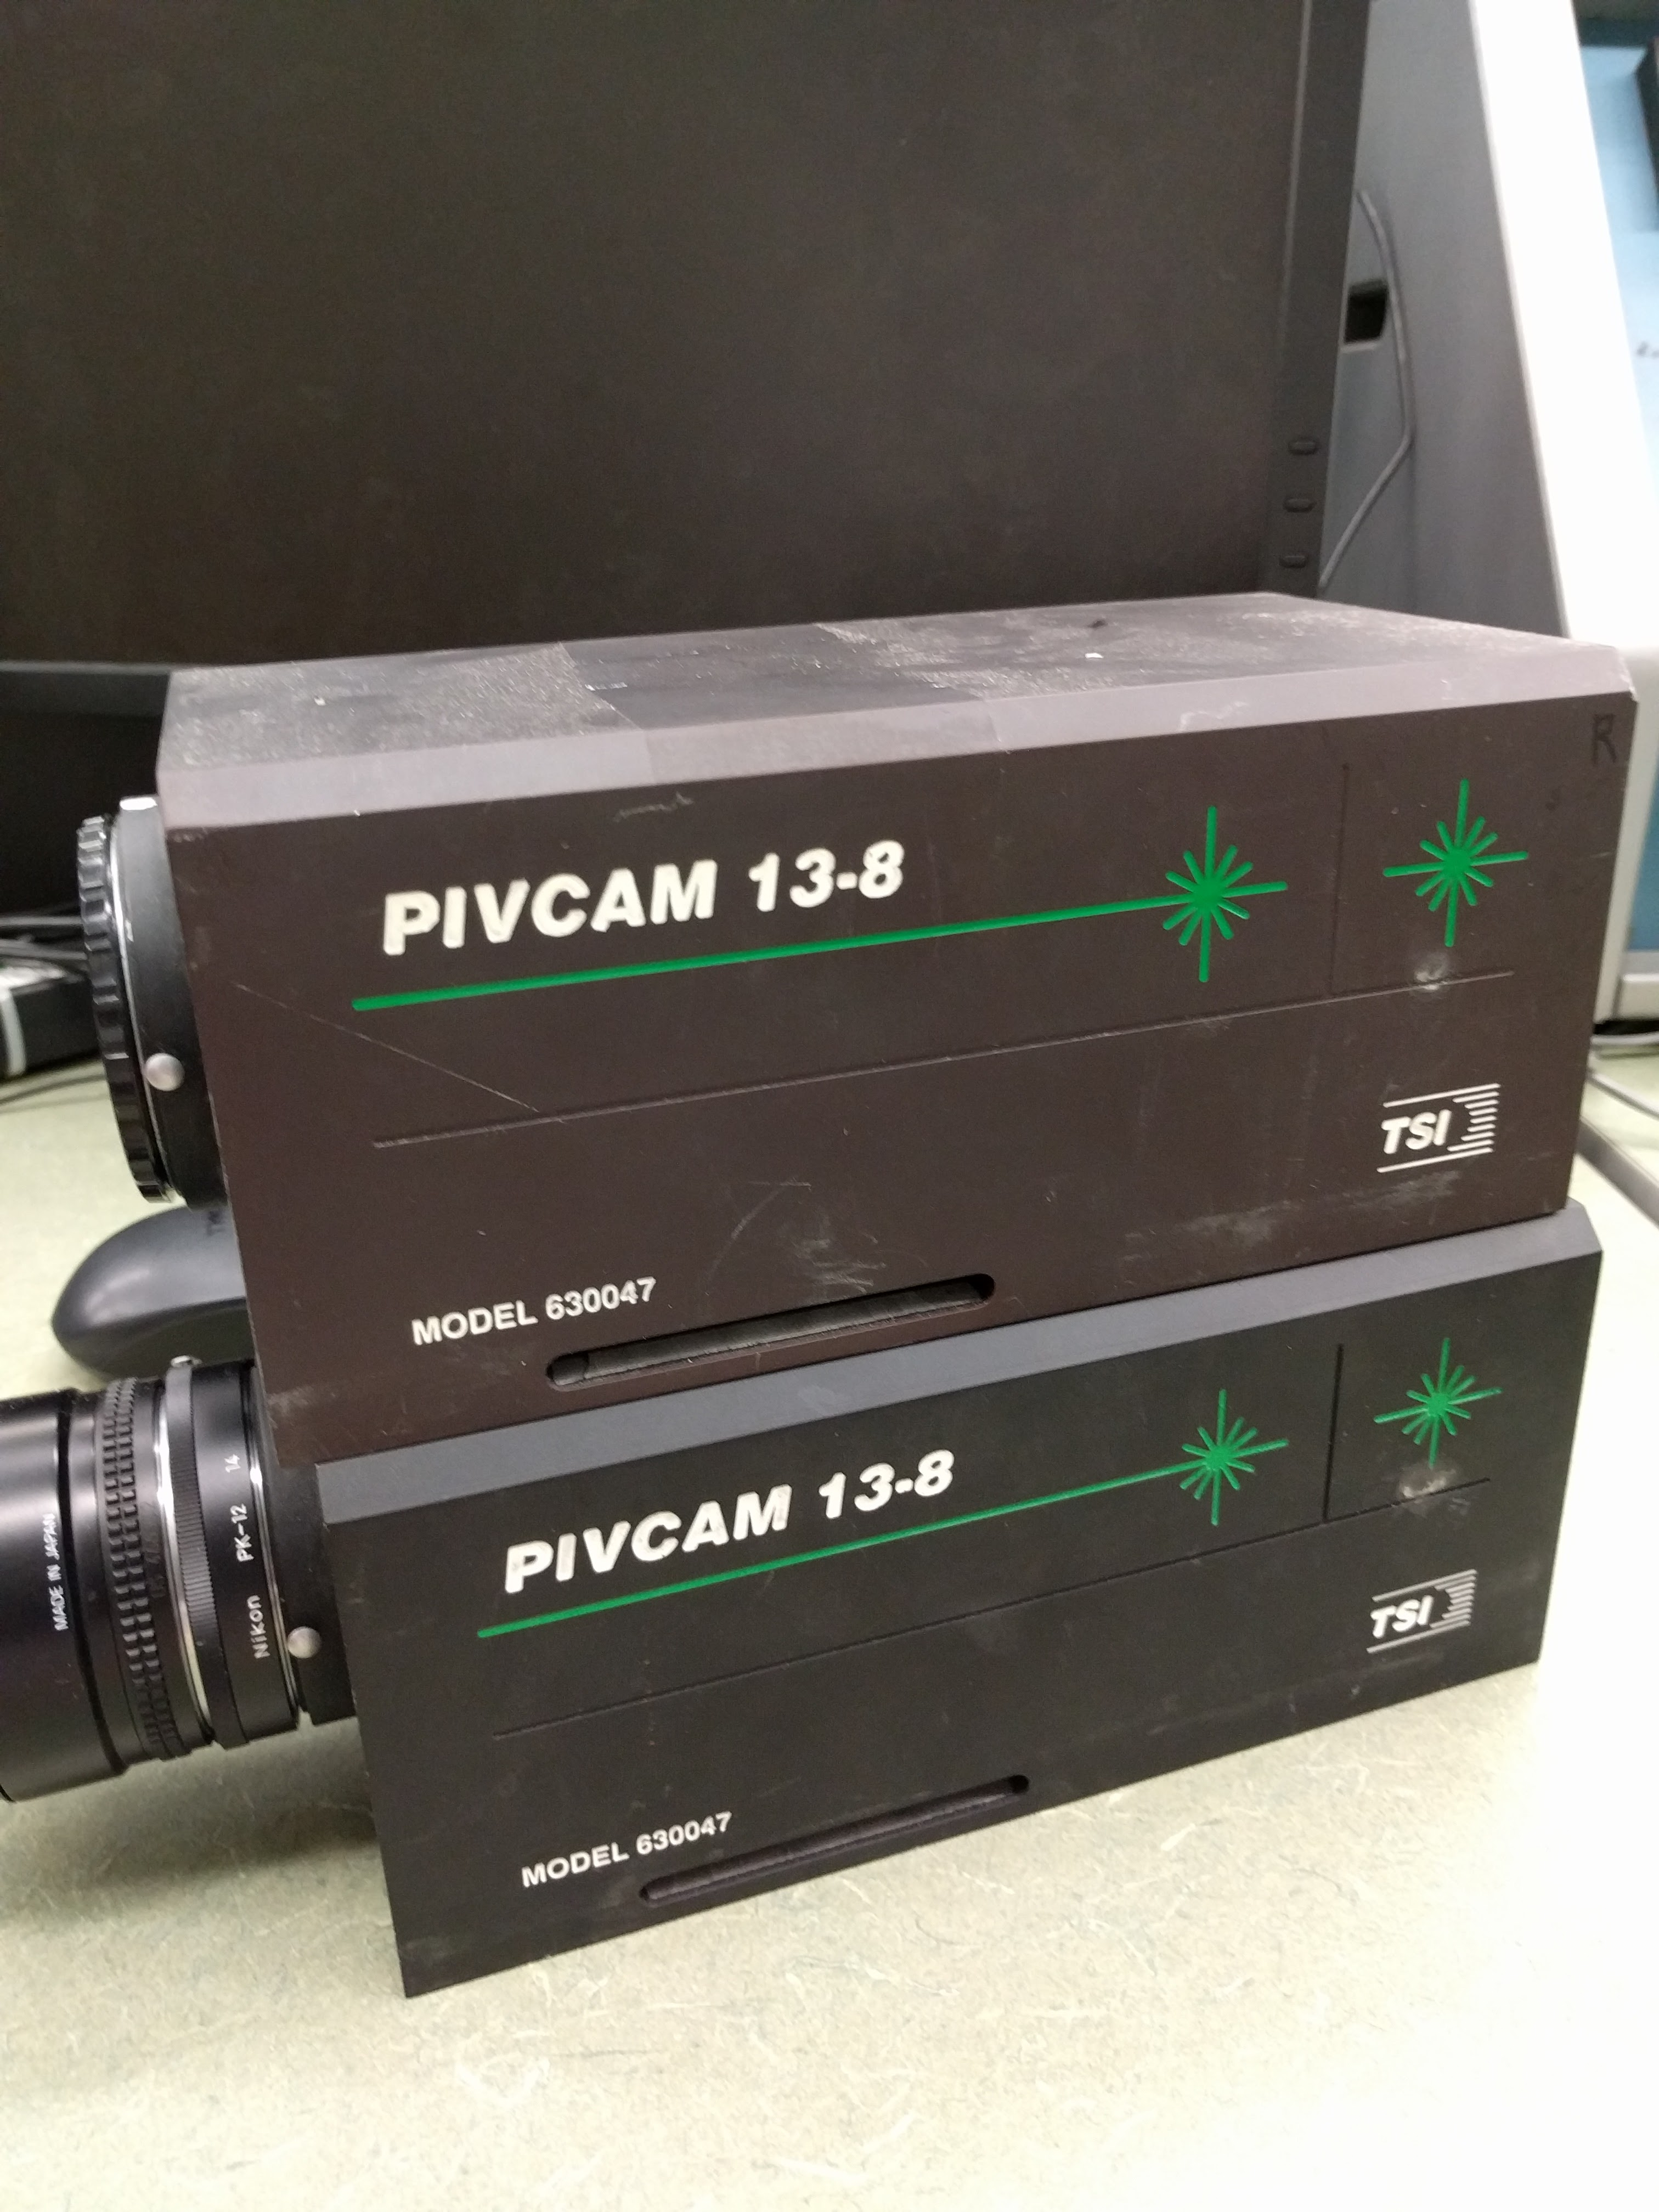
\includegraphics[width=5in]{figs/piv_method/piv_cams}
	\caption{Photograph of two TSI PIV 13-8 cameras. Model 630047}
	\label{fig:camera_picture}
\end{figure}

\begin{figure}[H]
	\centering
	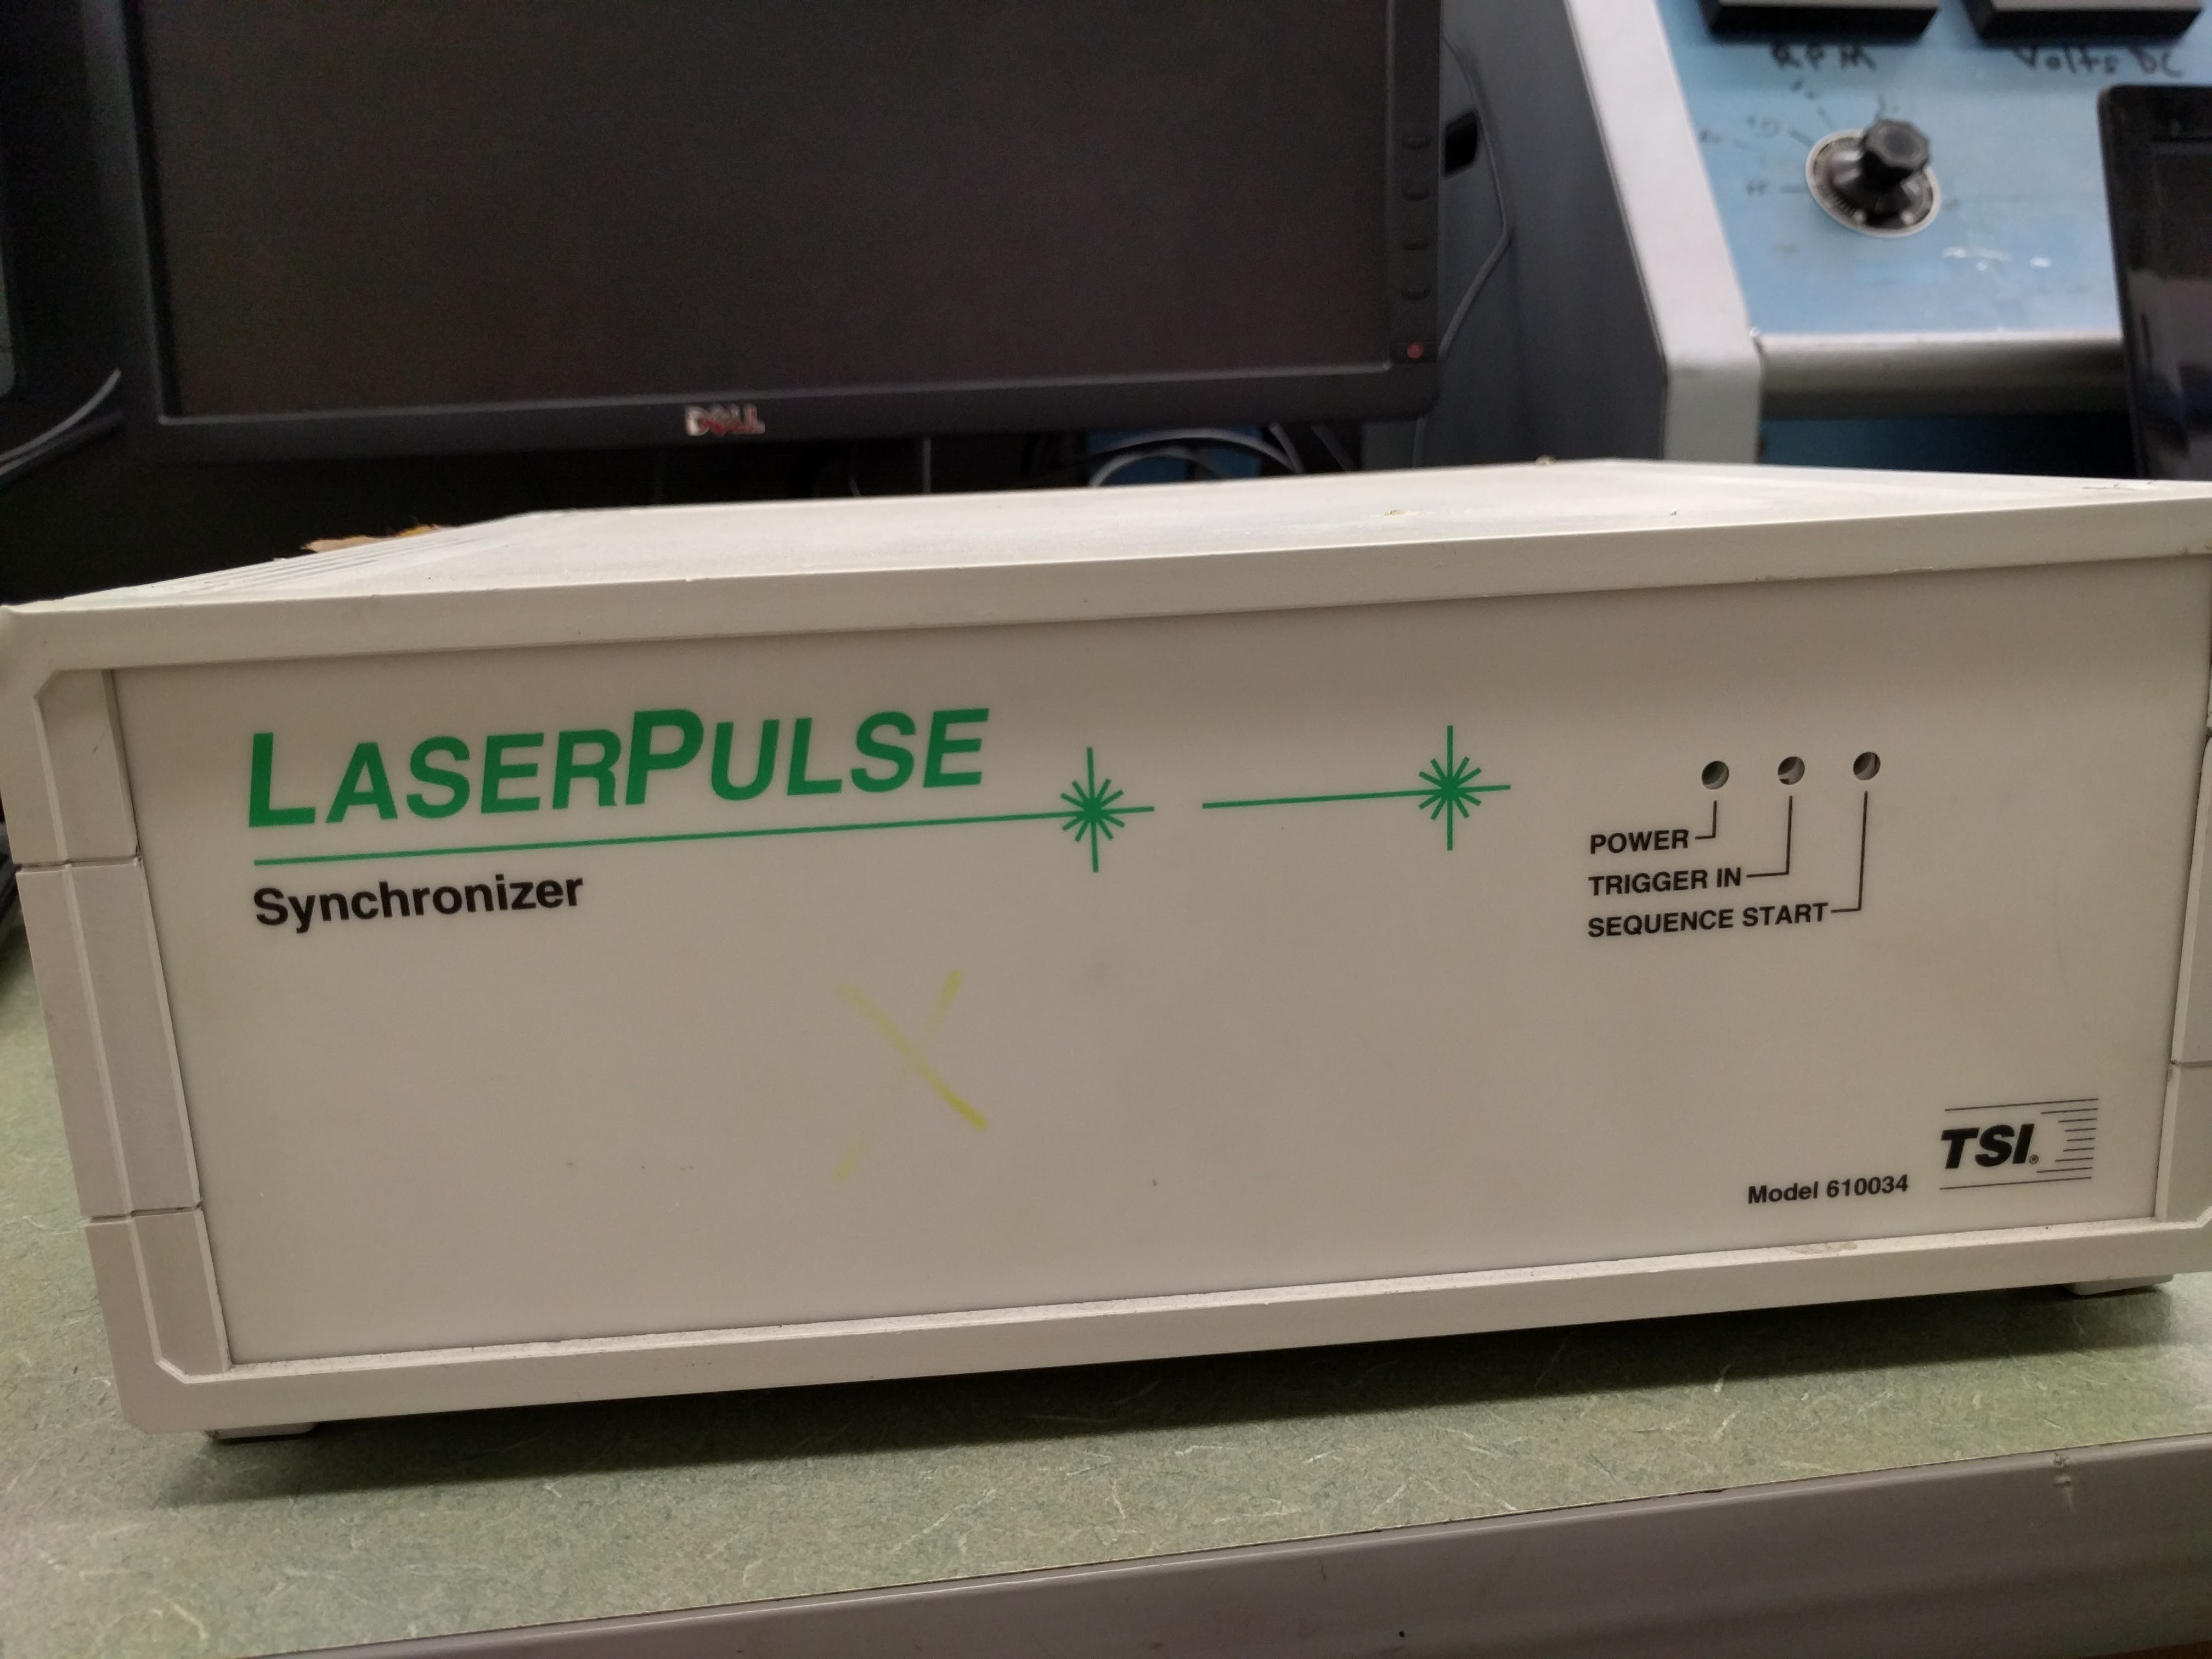
\includegraphics[width=5in]{figs/piv_method/synchronizer}
	\caption{Photograph of LaserPulse synchronizer by TSI. Model 610034}
	\label{fig:synchronizer}
\end{figure}

\begin{figure}[H]
	\centering
	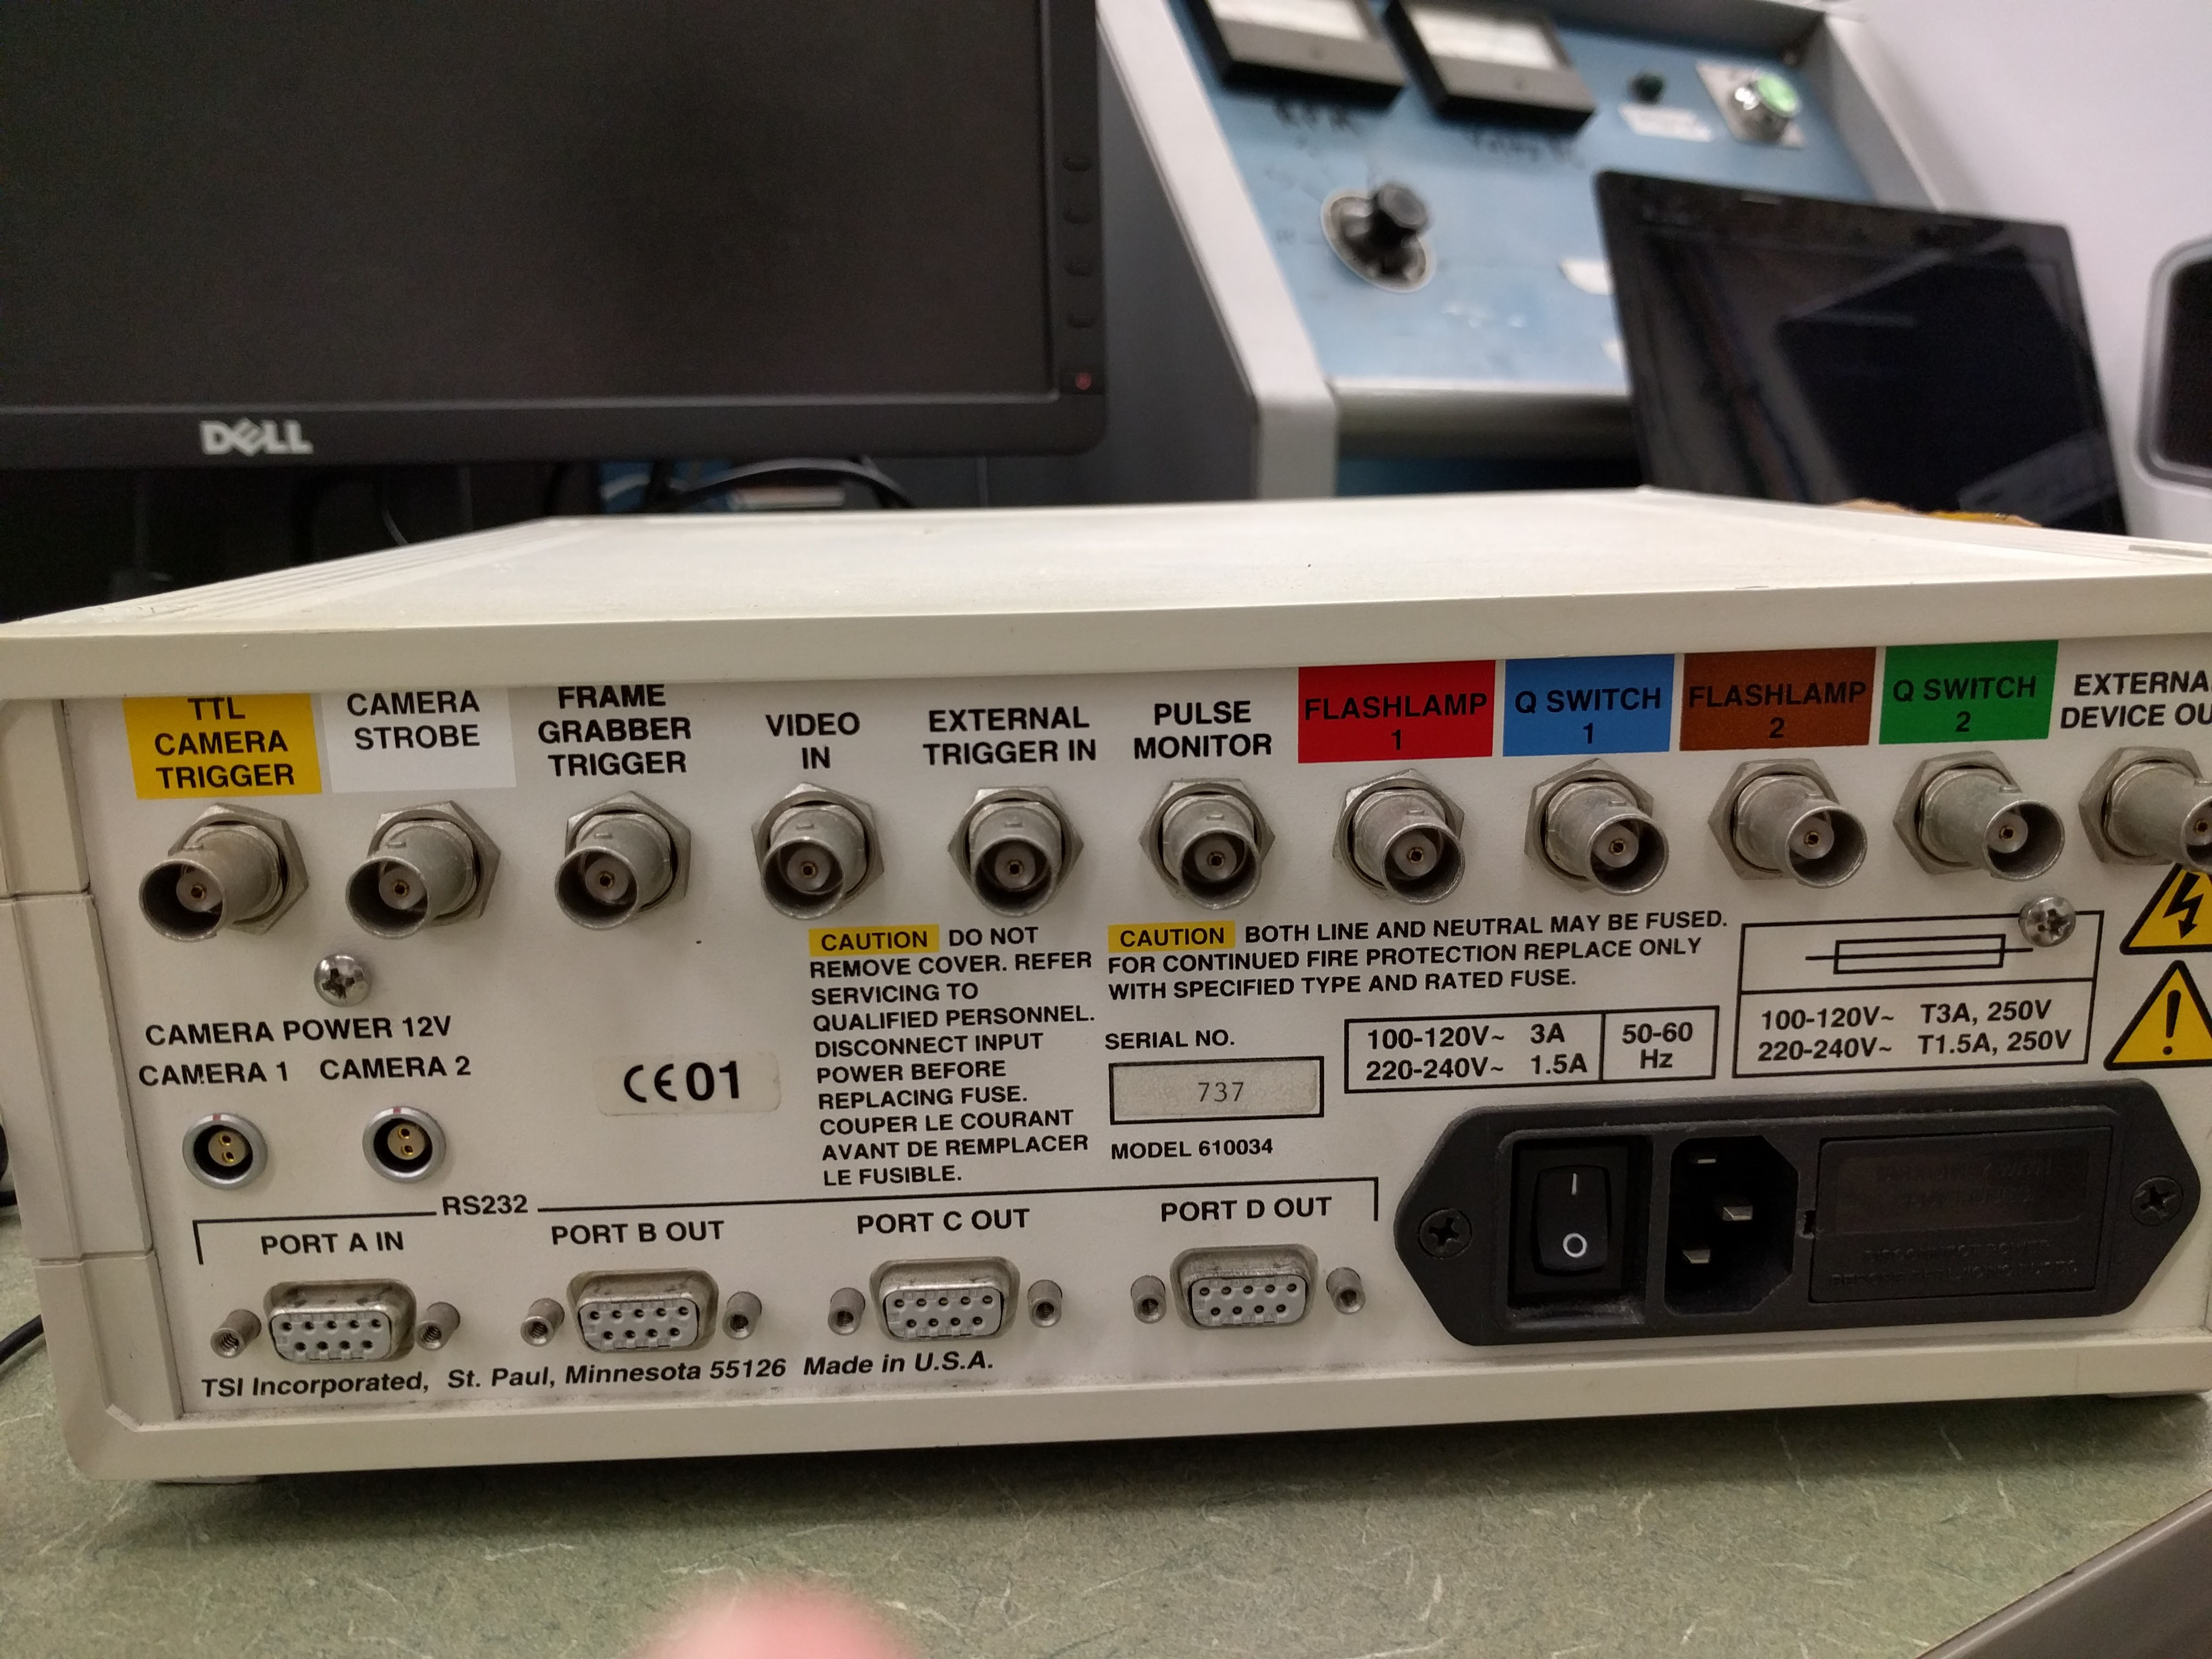
\includegraphics[width=5in]{figs/piv_method/synchronizer_rear}
	\caption{Photograph of synchronizer connectors. Model 610034}
	\label{fig:synchronizer2}
\end{figure}

\begin{figure}[H]
	\centering
	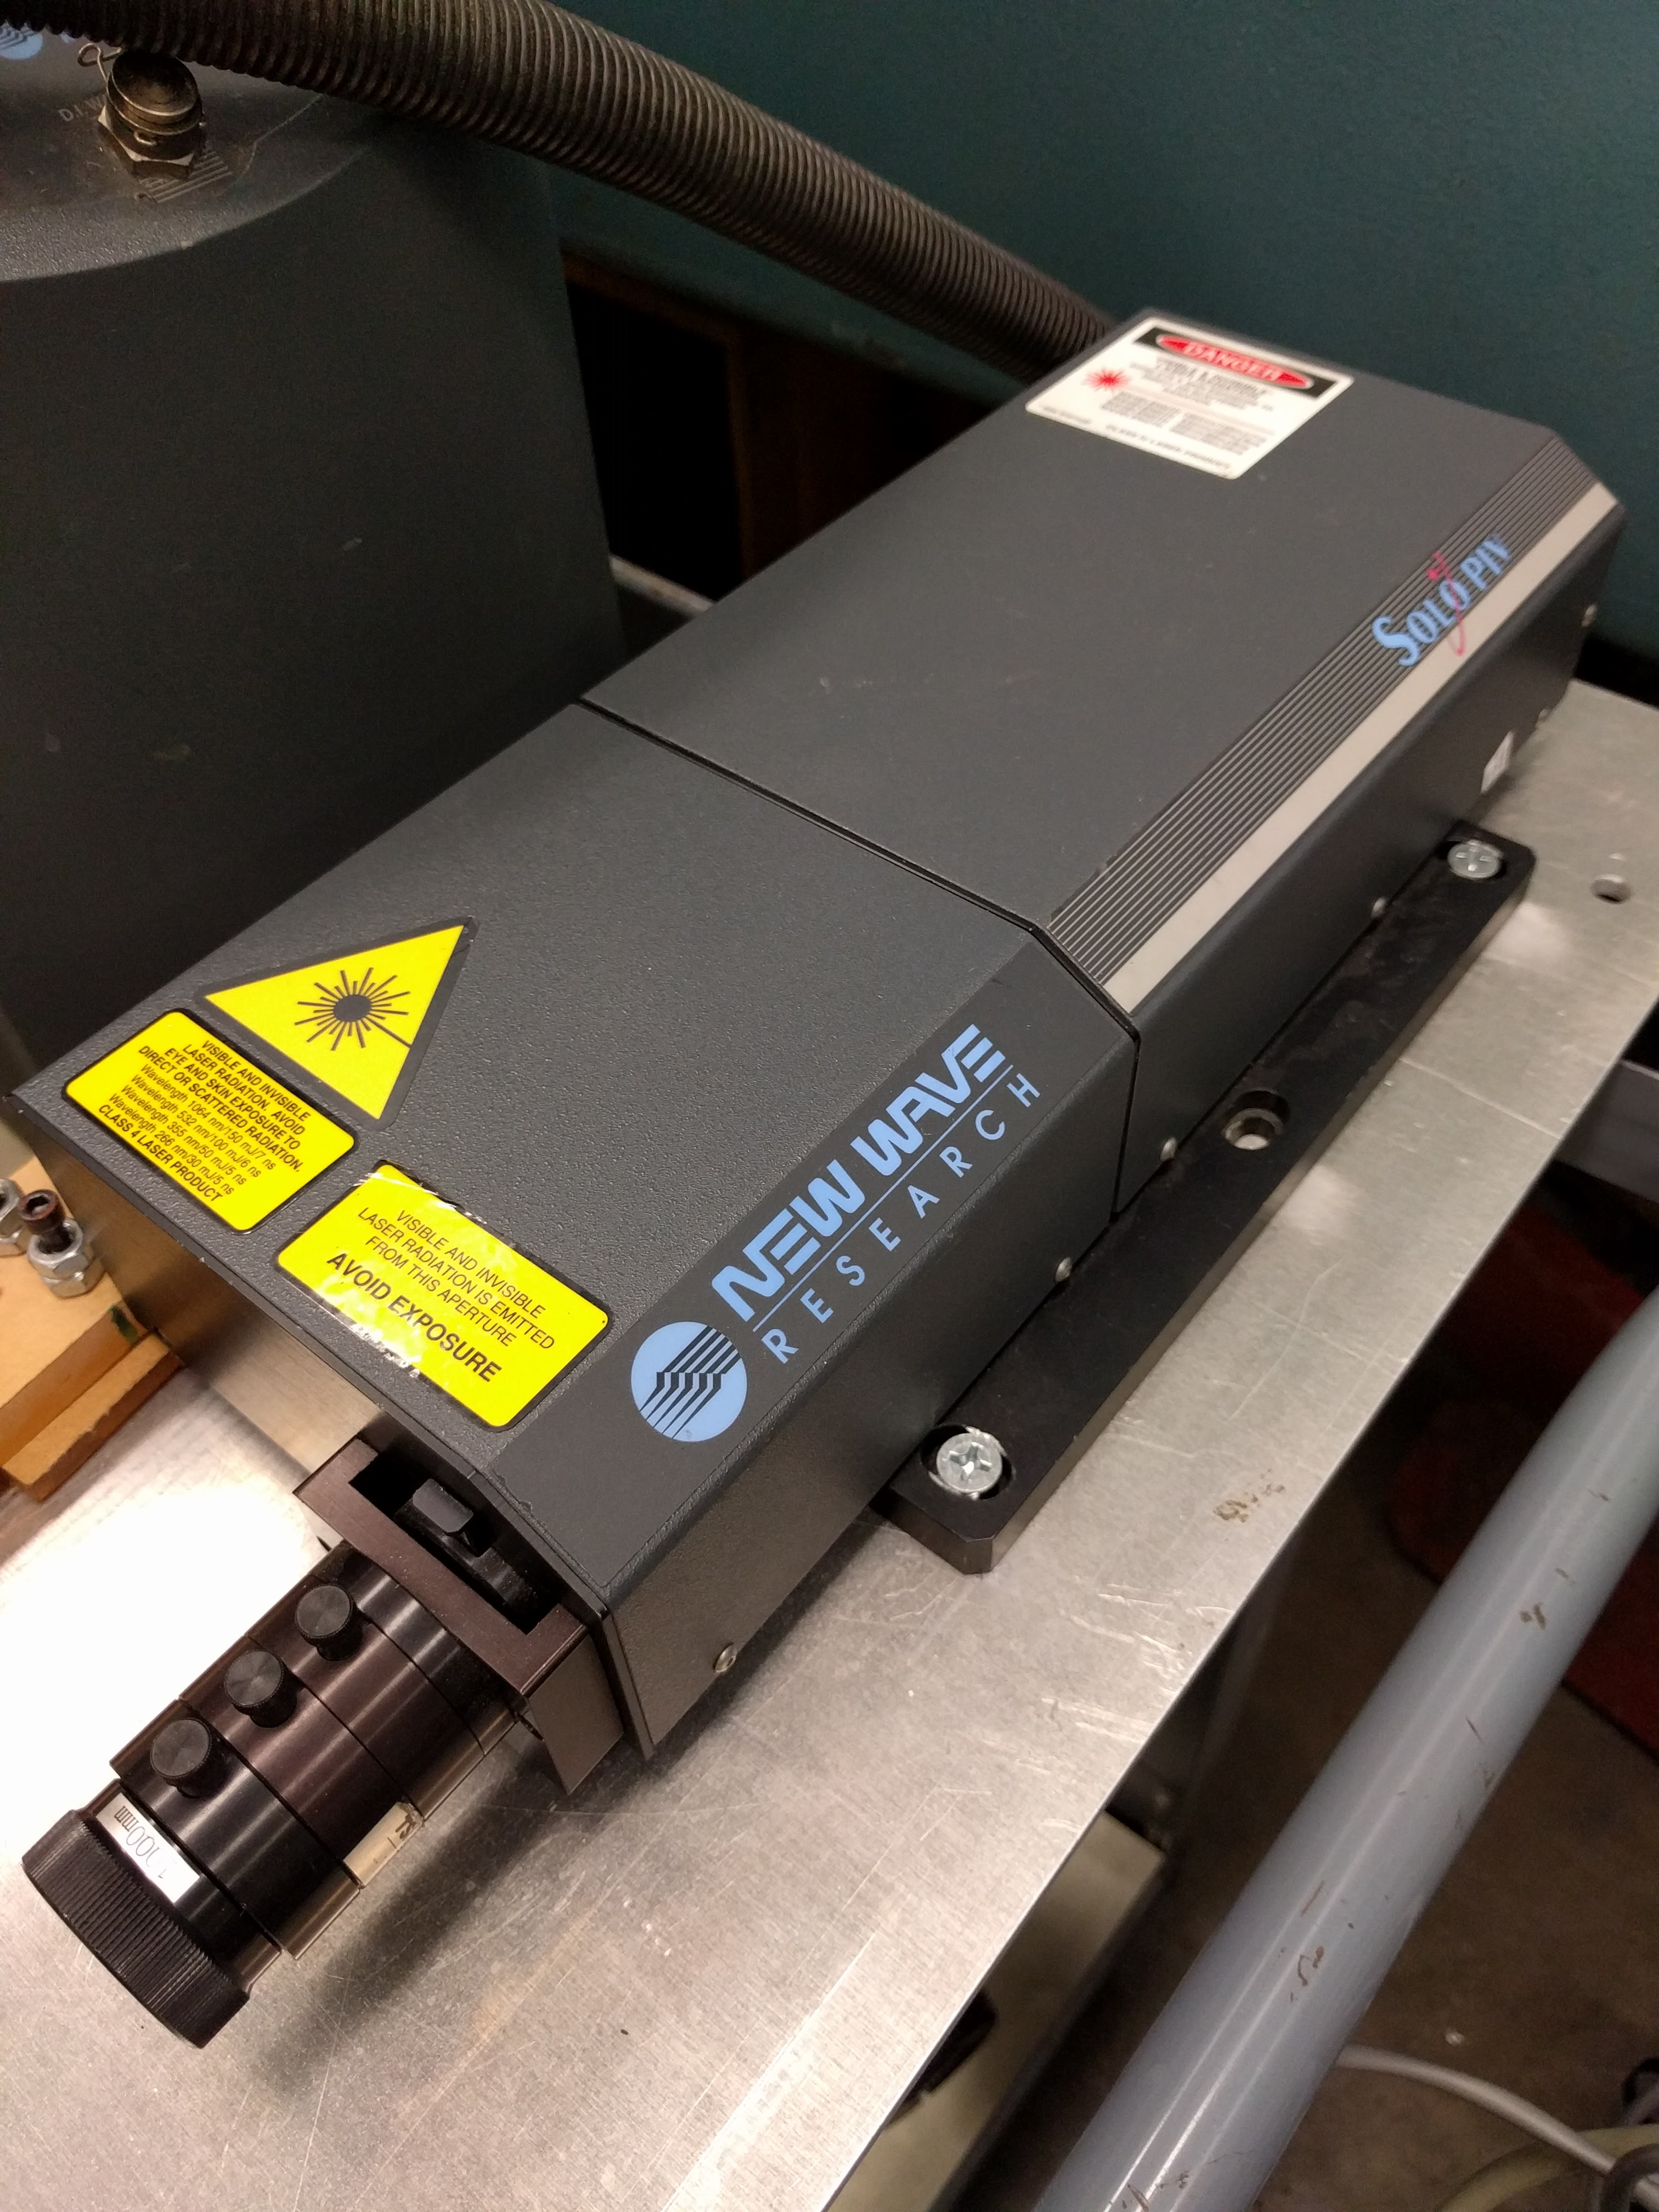
\includegraphics[width=5in]{figs/piv_method/laser}
	\caption{Photograph of a PIV laser by SoloPIV. Model 610034}
	\label{fig:laser}
\end{figure}

\begin{figure}[H]
	\centering
	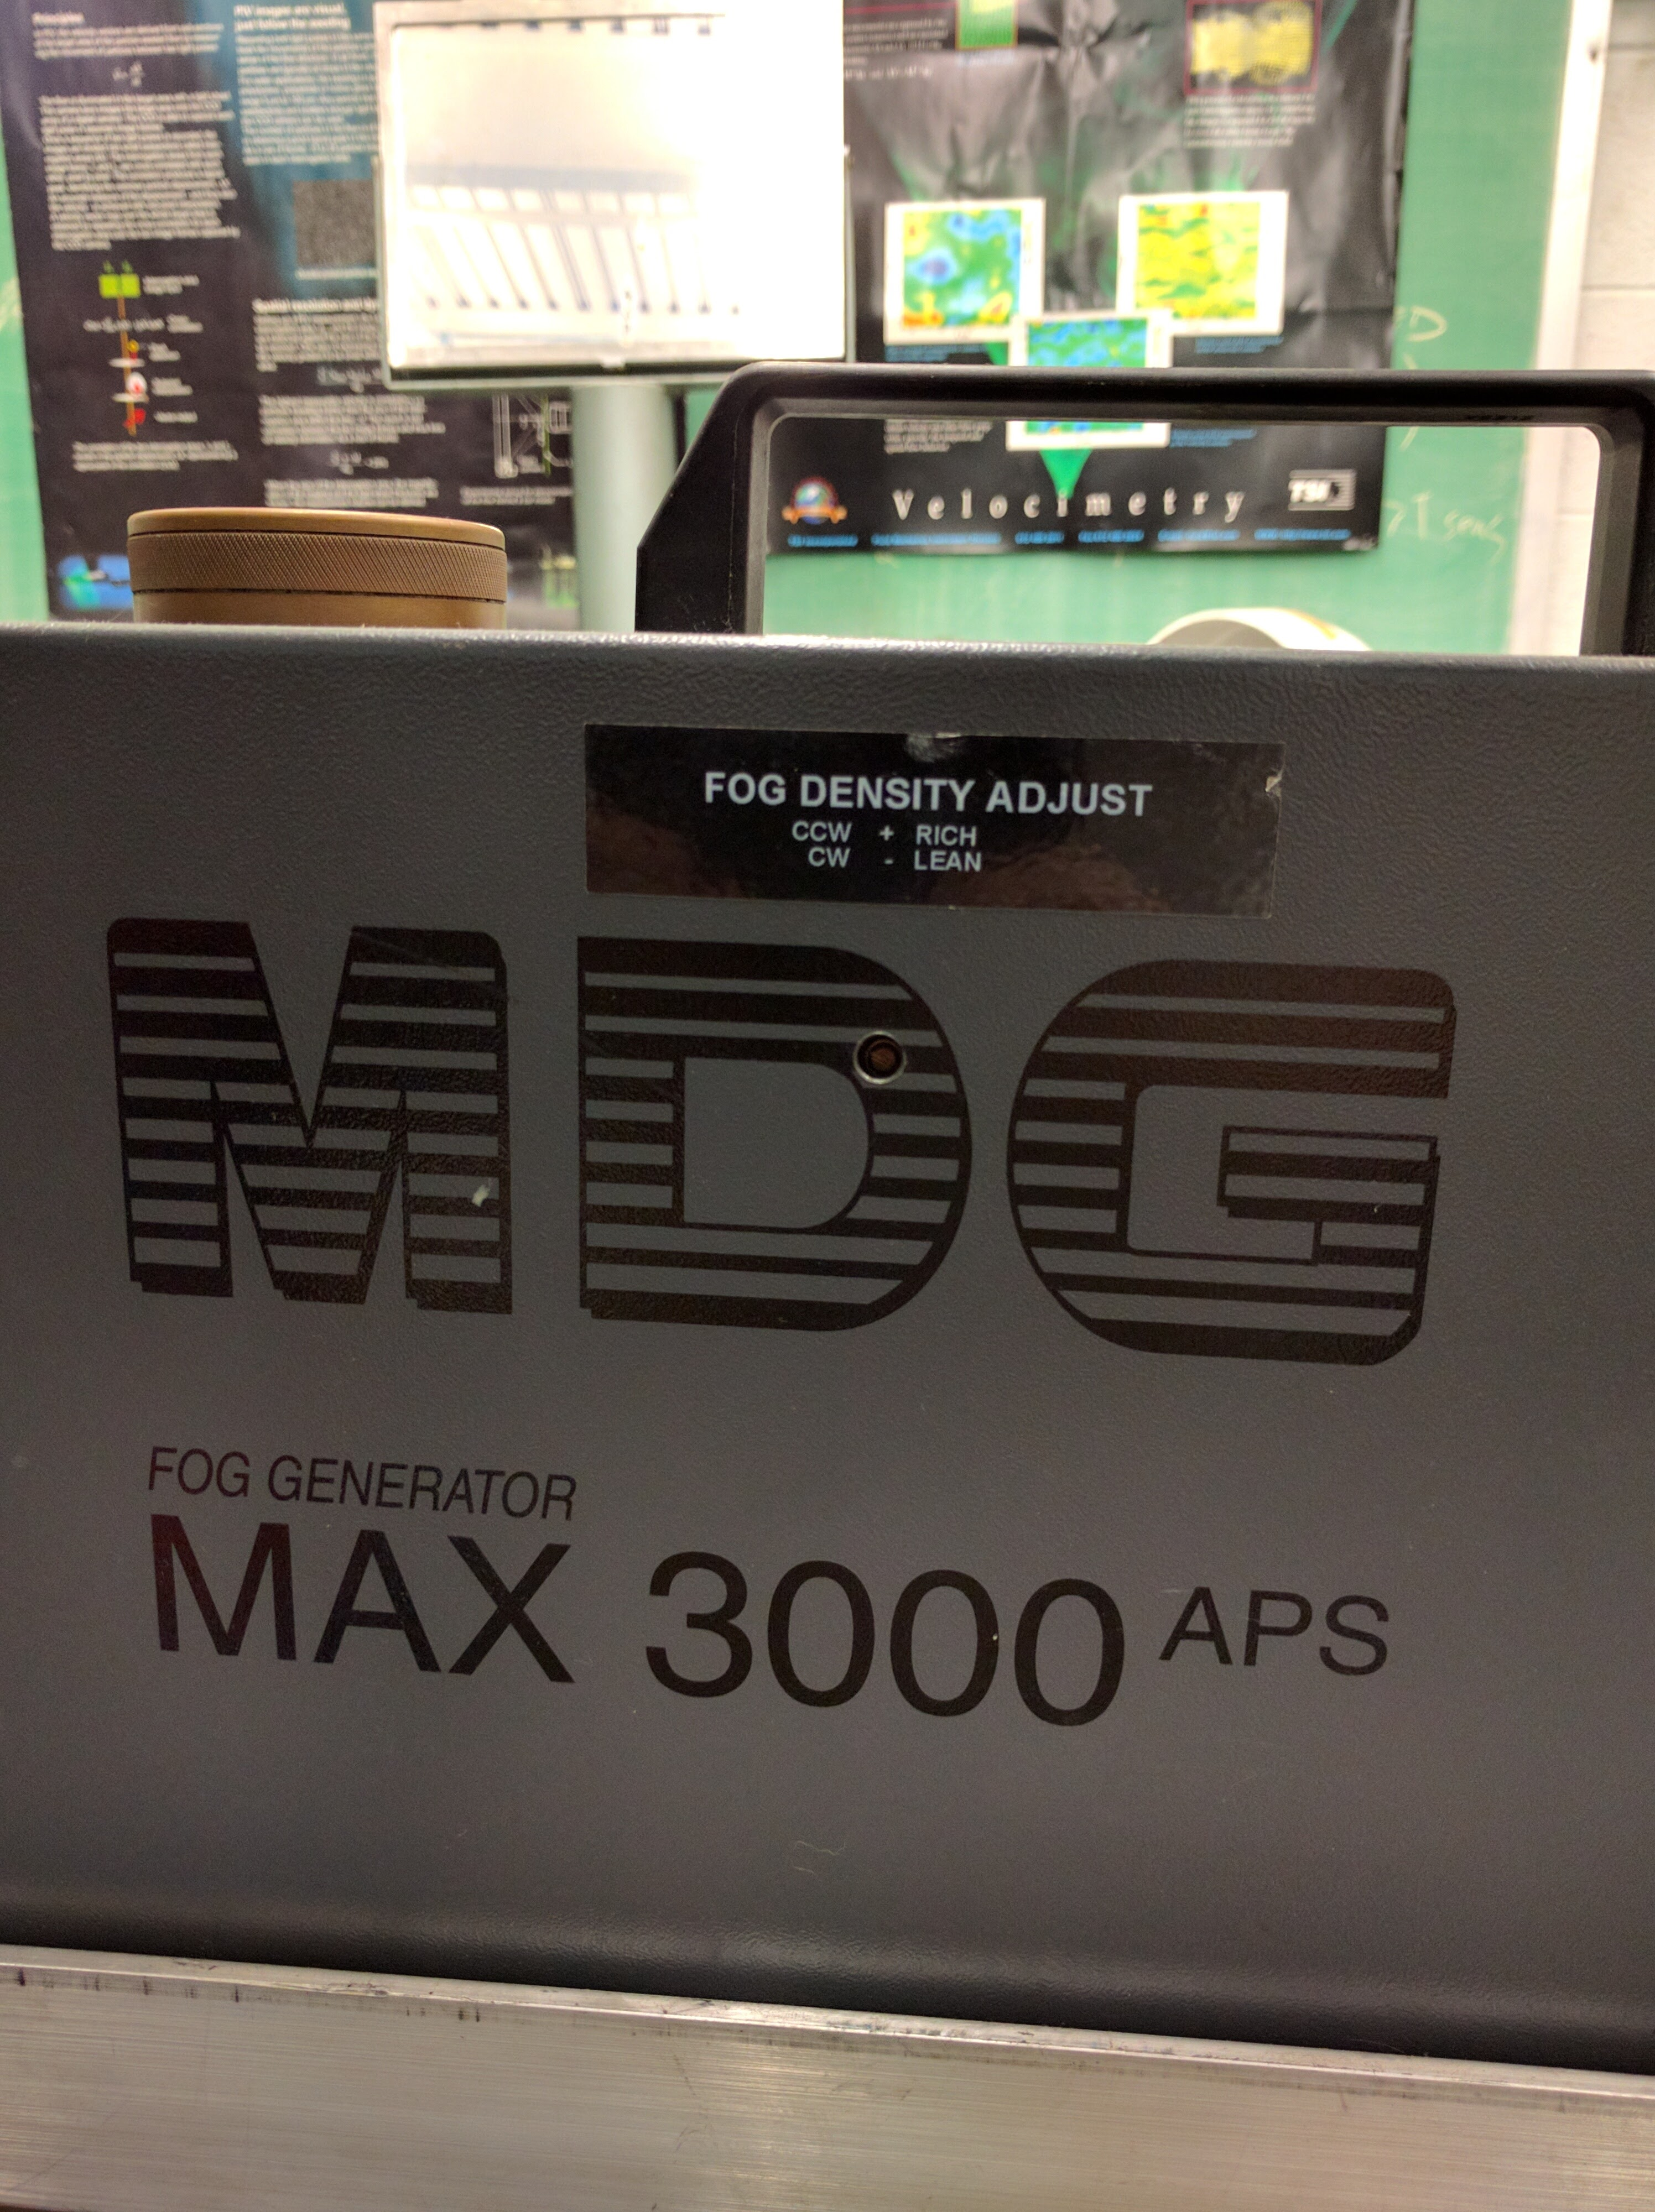
\includegraphics[width=5in]{figs/piv_method/fog_generator}
	\caption{Photograph MDG MAX 3000APS Fog Generator.}
	\label{fig:fog_machine}
\end{figure}

\begin{figure}[H]
	\centering
	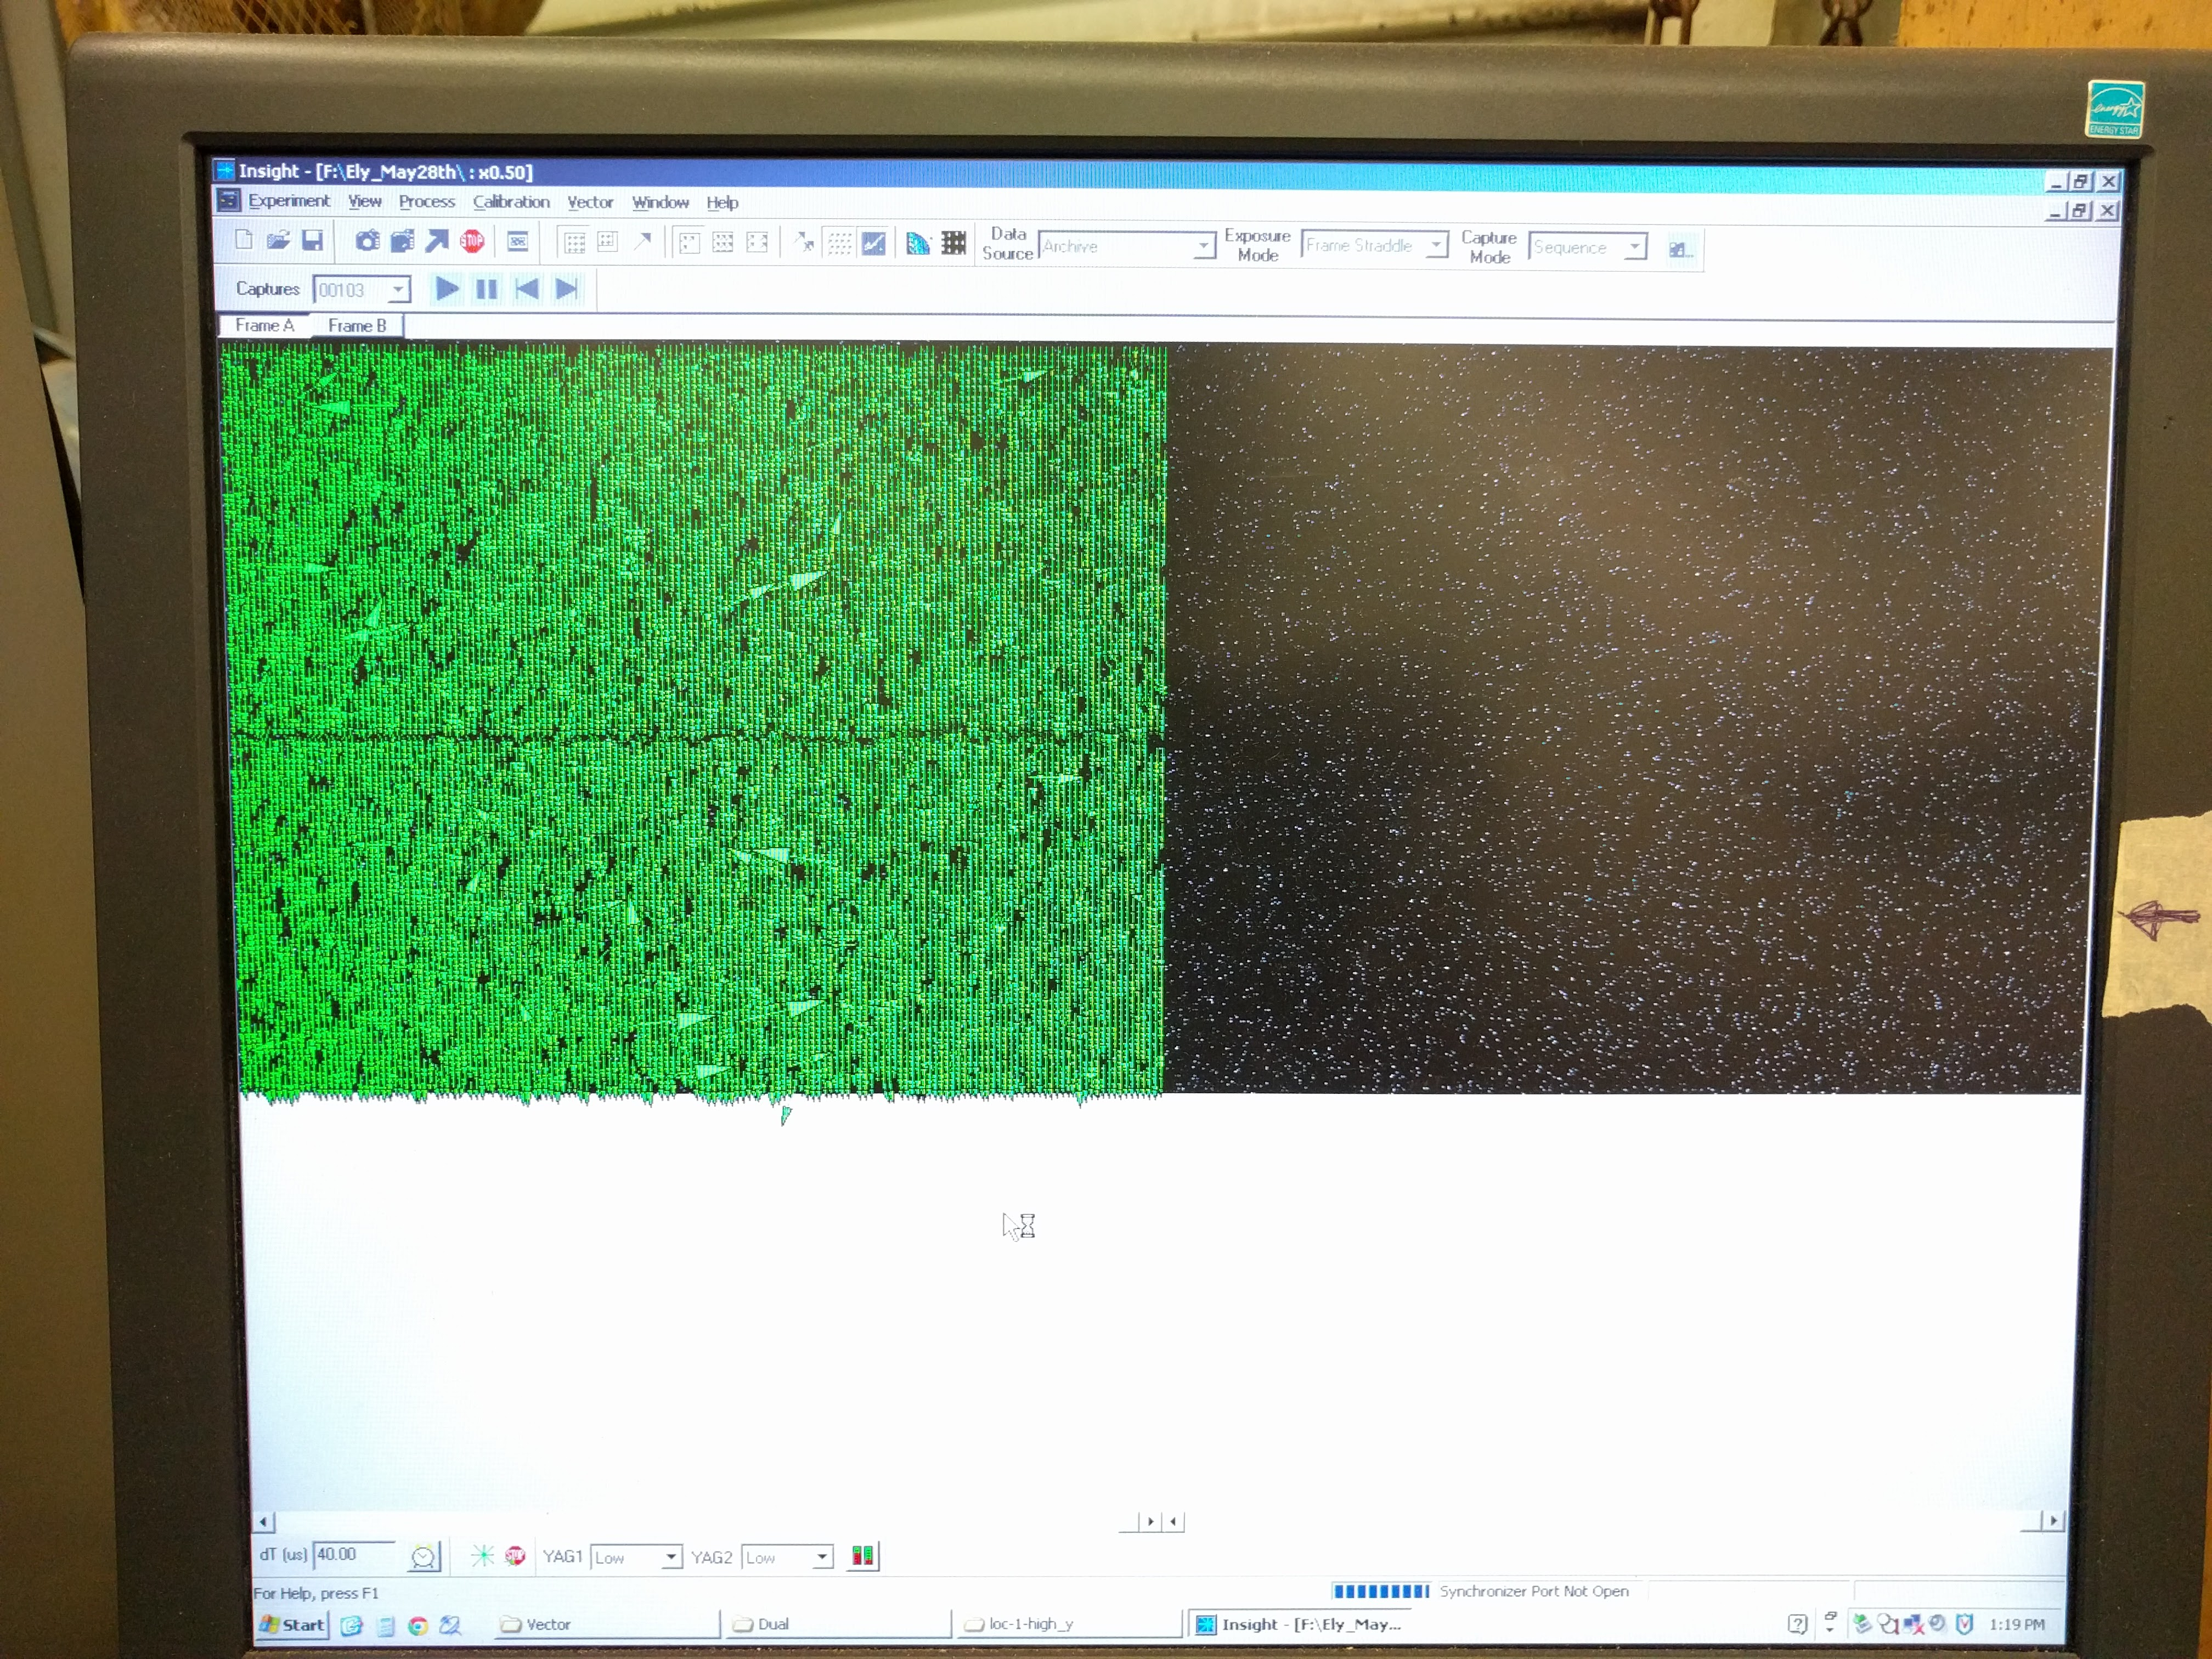
\includegraphics[width=5in]{figs/piv_method/INSIGHT_processing}
	\caption{Photograph of INSIGHT software computing stereo velocity fields}
	\label{fig:processing_screenshot}
\end{figure}

\subsection{Synchronizing the Cameras and Laser}
In order to resolve particle displacements on such a small scale in a 
relatively fast moving fluid, the time between a pair laser pulses must be 
tuned to allow sufficient particle displacement occur to obtain a meaningful 
velocity measurement. If the time interval ($dT$) between successive exposures 
was too long, the particles escape the interrogation plane, and cannot be 
tracked to measure their displacement. This study varied the laser pulse timing 
between 25 microseconds for higher wind tunnel speed, and 50 microseconds for 
slower vortices associated with slower wind tunnel speed. The cameras used for 
these experiments however could not support an exposure time on the order of 
microseconds, consequently a frame straddling technique was used. Frame 
straddling initiates the first shutter opening well before the first laser 
pulse begins such that the camera shutter first closes at as the first laser 
pulse is ending, but before the second laser pulse starts. The second exposure 
begins just as the second laser pulse is initiating, though it extends well 
beyond the termination of the first laser pulse as shown schematically in 
Figure \ref{fig:frame_straddling}. 

\begin{figure}
	\centering
	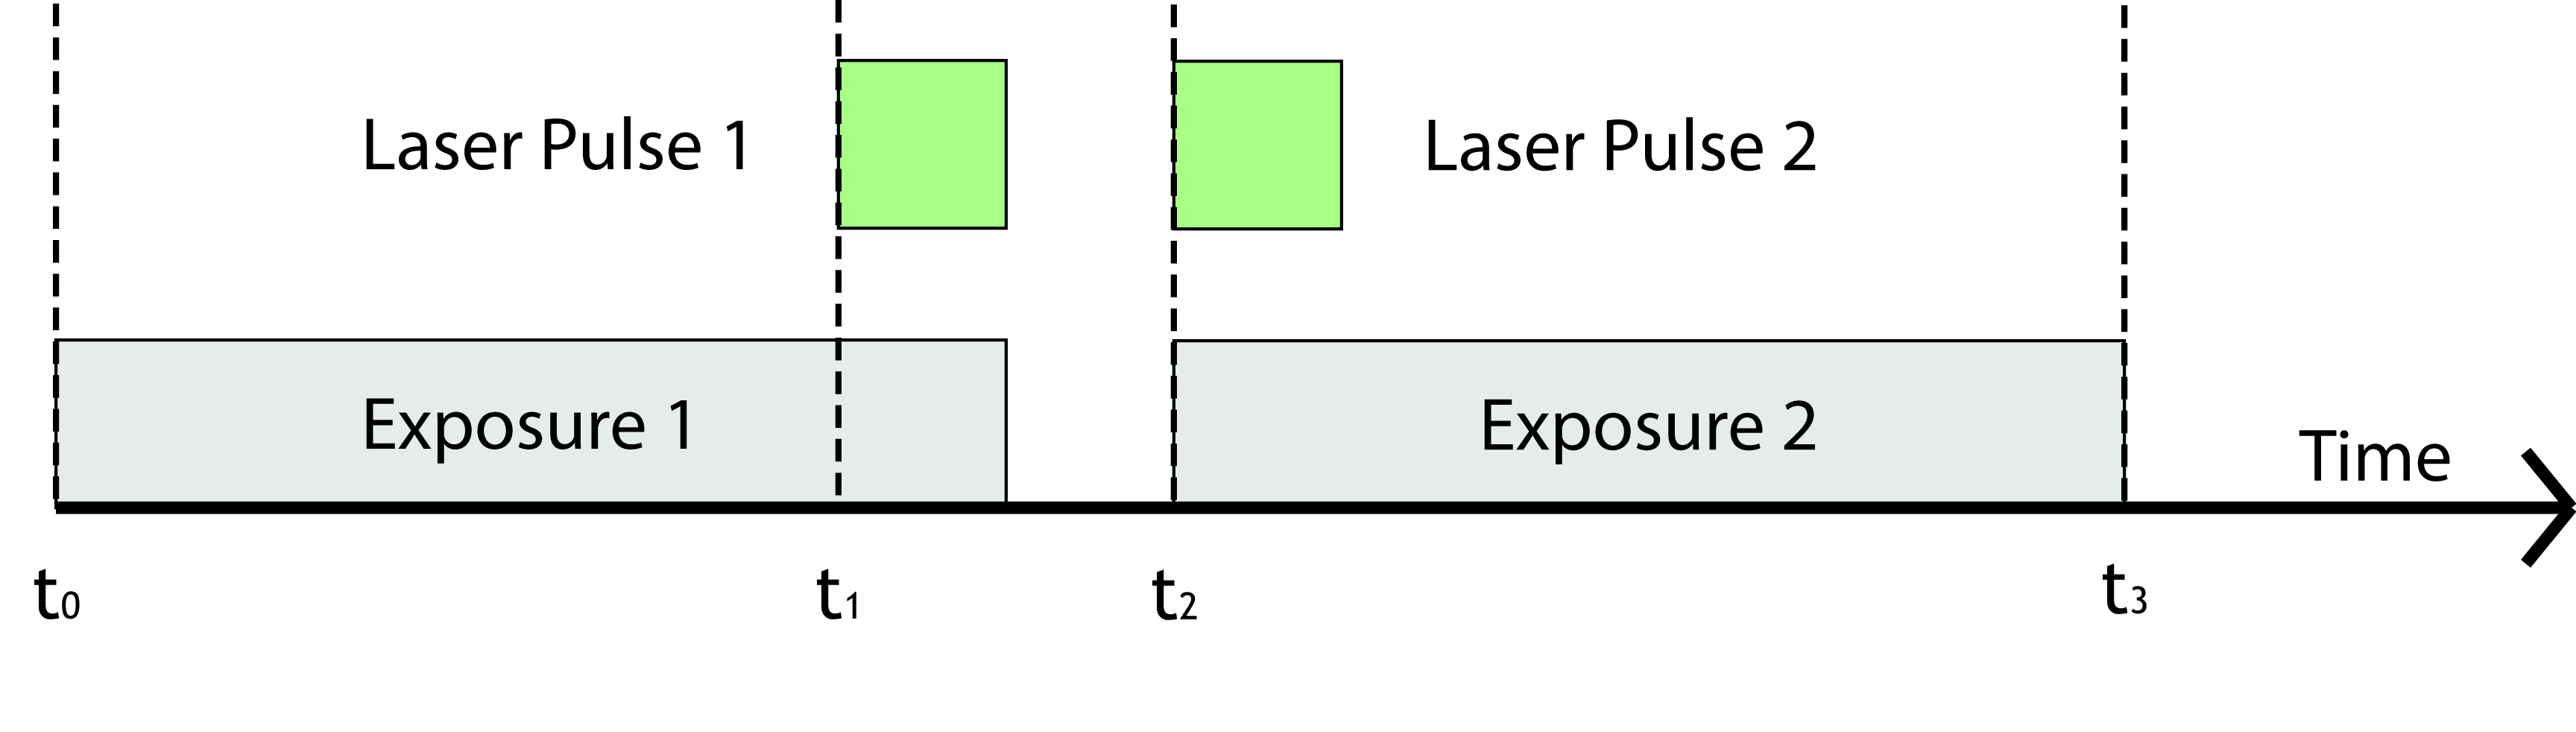
\includegraphics[width=5.5in]{figs/piv_method/frame_straddling}
	\caption{Frame straddling technique. Laser pulses are shown in green, and 
		camera exposures are shown in gray.}
	\label{fig:frame_straddling}
\end{figure}

Timing is achieved by the synchronizer and control PC shown in figure 
\ref{fig:pivblockdiagram}. The control PC sends a command to the synchronizer 
to take an image sample, then the synchronizer sends precisely timed signals to 
both cameras and the laser control unit. The cameras each store the image pair 
in an internal memory buffer before returning the data to the control PC.

\begin{figure}[H]
	\centering
	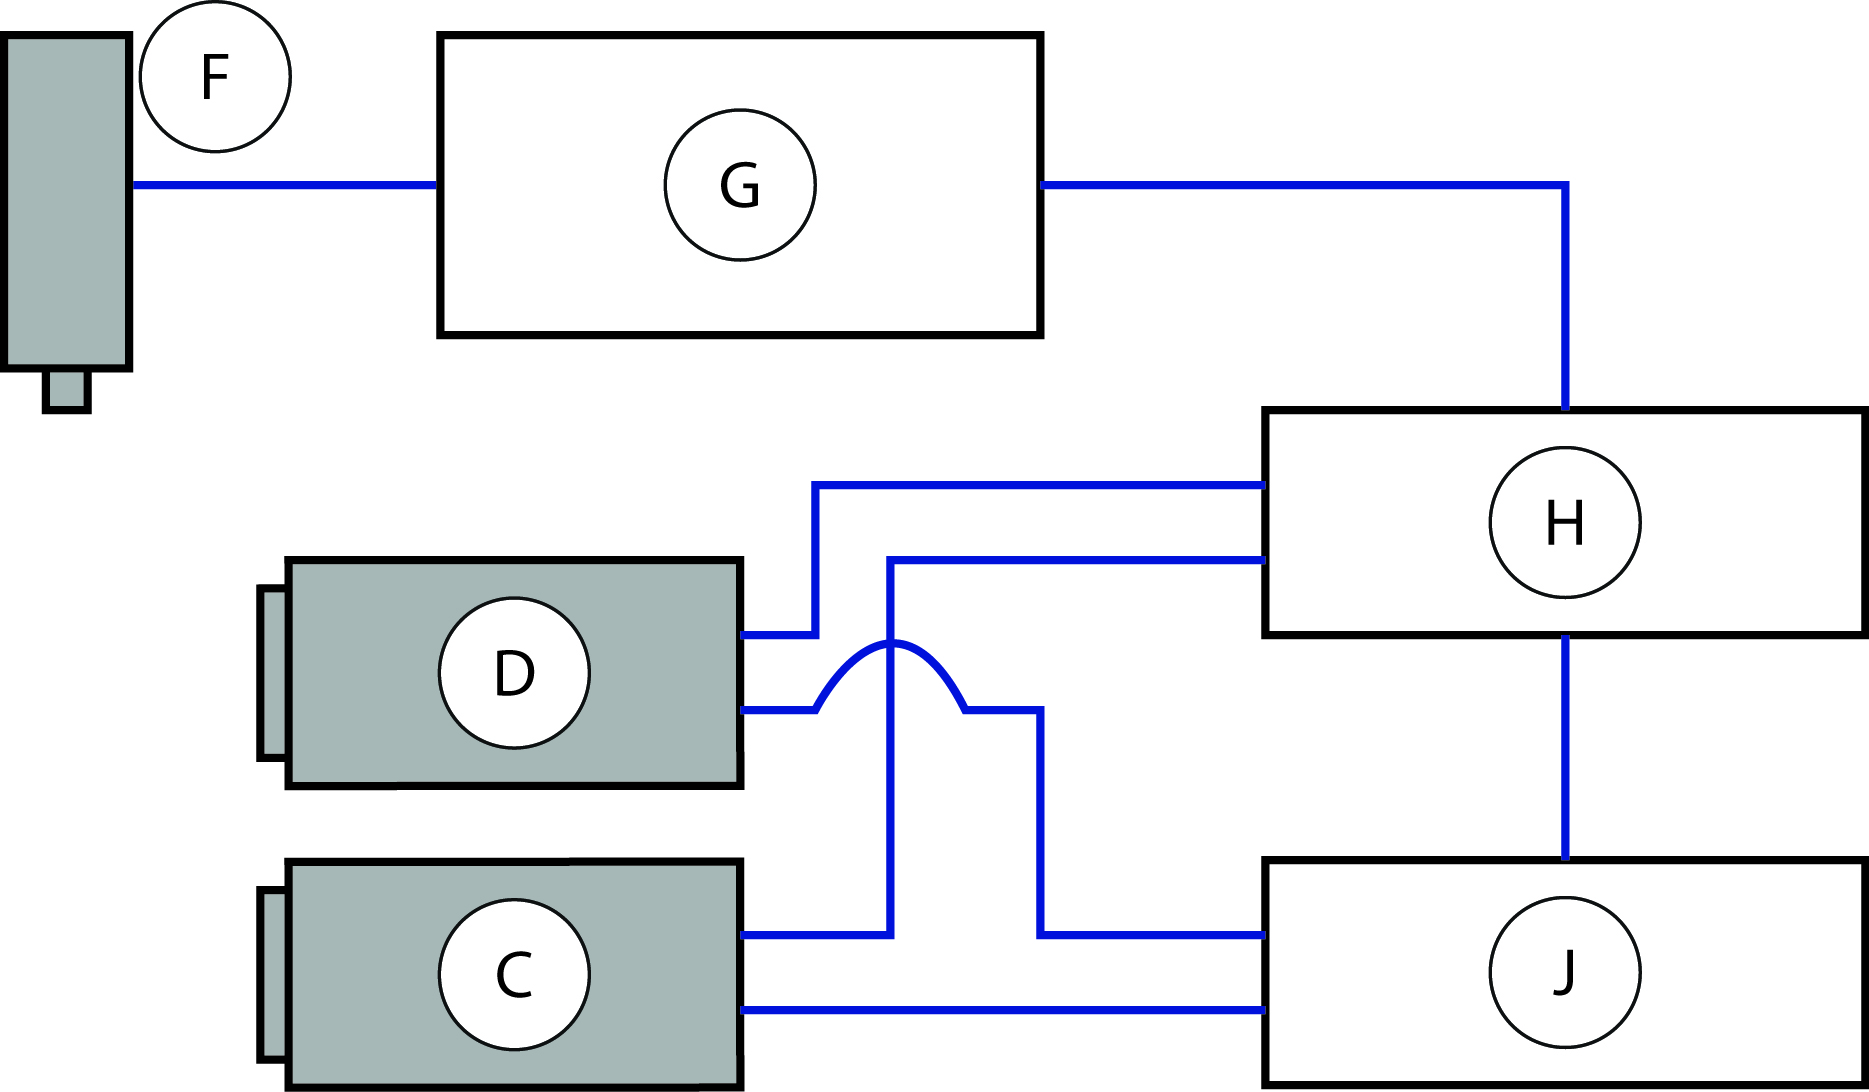
\includegraphics[width=4in]{figs/piv_method/experiment_block_diagram}
	\caption{Blockdiagram of PIV hardware components. C-left camera, D-right 
		camera, F-Nd:YAG laser, G-laser control unit and power supply, 
		H-synchronizer, 
		J-control PC running INSIGHT software suite.}
	\label{fig:pivblockdiagram}
\end{figure}

\subsection{Calibration employing a PIV Target}

Dimensional calibration is accomplished with the use of a calibration target, a 
10$cm$ by 
10$cm$ black calibration target with precisely positioned white divots and a 
center fiducial mark ,as shown in figure \ref{fig:calibration_target}. The 
calibration target is 
positioned inside the tunnel test section and aligned with the desired 
interrogation plane. 
The laser illumination sheet is set to a continuous firing mode and aimed into 
the test section so that the location of the interrogation sheet is clearly 
visible with the use of polarized eye protection. The camera facing face of the 
interrogation target is then manually aligned with the interrogation plane, 
which is visible as an intense line of light with a nominal thickness of 
1.5$mm$ across the top of the target. Once the calibration target was properly 
aligned, the laser and all other light sources in the facility were 
extinguished and a lamp is placed downstream of the test section (to create 
ideal lighting conditions) and illuminate the target for camera focusing. 
Cameras outfitted with 50mm lenses were manually aimed at the calibration 
target, taking 
care to place the fiducial mark near the center of the frame. Focusing must 
also be done manually by adjusting each lens, and a limited PIV data set was 
taken after focusing to ensure the focus is sharp enough to resolve a partially 
complete velocity vector field within the interrogation plane.

\begin{figure}[H]
	\centering
	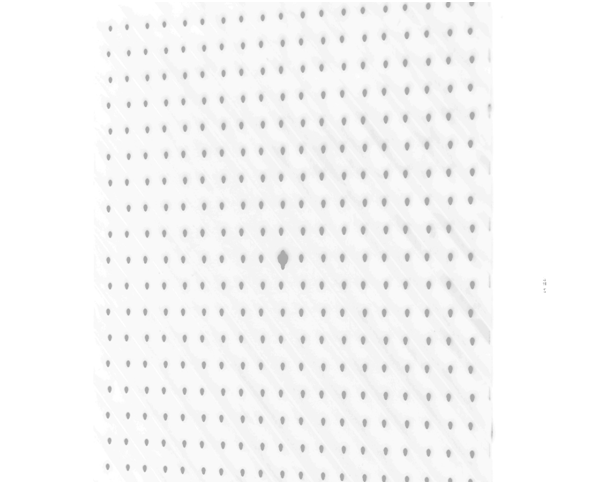
\includegraphics[width=4in]{figs/piv_method/calibration_target}
	\caption{Inverted color and elevated contrast photograph of the calibration 
		target, highlighting the central fiducial mark.}
	\label{fig:calibration_target}
\end{figure}


INSIGHT software was used to take snapshots and view them to ensure proper 
focus 
and alignment. Once satisfactory adjustments were obtained, calibration images 
were taken and the imaging software was used to recognize the fiducial mark, as 
well as each divot, in order to create a two dimensional coordinate transform 
map that relates 
pixel distance to physical distance. This calibration was used both in 
determining the magnitudes of the two dimensional vector fields unique to each 
camera, and aligning the two separate vector fields, in order to create a three 
dimensional velocity field. Once calibration images have been acquired, the 
target 
was removed from the tunnel and data were taken over a range of velocities in 
that interrogation plane. Each interrogation plane is defined by its position 
downstream relative to the trailing edge of the vortex generator. Several 
interrogation planes were required, and every time it was changed, it was 
necessary to repeat the calibration process. Ideally, as dictated by good 
design of experiments 
practice, the order of experiments should be randomized. This, however, would 
have required exclusive tunnel use for a longer period of time than could be 
scheduled due to the level of demand at the time.

\subsection{Seeding the Flow}

Gathering data with a PIV system requires the flow be properly seeded with 
particles. Particles should be sufficiently small to be entrained in the flow 
such that particle motion and fluid motion are the same. The low speed wind 
tunnel uses mineral oil fog as seed. The density of particle seed which 
produces the most complete PIV data set depends upon the free stream velocity 
and 
the spacing between velocity vector measurements. Each velocity measurement 
requires a sector of pixels through which displacement can be tracked. If 
a majority of particles are allowed to travel outside of a given 
sector between consecutive frame straddled image captures, a meaningful 
correlation map cannot be 
generated. Care is taken to ensure particles travel no more than 50\% of a 
sector width during the time interval between images by adjusting the time 
between image captures ($dt$). 
Utilization of a 50\% border when processing each sector, as described in the 
previous section, helps to ensure particles do not escape the interrogation 
area. A sufficient quantity of particle groups must be visible in each sector 
to yield a meaningful correlation map. If the particle seed density is too low, 
or too high, it will result in a more homogeneous image, with more ambiguous 
and peaks in the correlation map, which results in more spurious data with a 
poor signal to noise ratio. Manipulation of sector size 
can increase the number of particles and the reliability of the correlation 
mapping, but only at the expense of velocity field resolution, as more pixels 
are required to resolve each vector.


\subsection{Pressure Measurements}

Pressure measurements within the vortex core could assist in demonstrating the 
applicability of pressure relaxation pheneomenon in describing the behavior of 
an axial wave vortex, especially combined with simultaneous three-dimensional 
turbulence measurements with PIV \cite{ash2011}.
Initially, it was believed that a pressure probe could be positioned 
inside the flow within the vortex core. Without positioning the probe in many 
locations across the flow and post-processing the data set, it was necessary to 
have some other way to verify that the pressure probe was in fact positioned 
within the vortex core. Simultaneous PIV and pressure measurements were 
attempted with a seven hole probe, but the probe and probe mounting system was 
found to severely obstruct the PIV laser sheet and camera views, and created 
bright reflections that saturated image values in the vicinity of the vortex. 
No usable PIV data could be taken while a pressure probe was mounted in the 
tunnel test section. Furthermore, upon direct visual inspection of the live 
vortex core employing a continuous laser sheet, the core appeared to dilate 
significantly in 
the presence of the pressure probe. 
Without a method to compensate for this 
potential core dilation, pressure measurements of the vortex core region could 
not be included in the final experiments of this study. It is possible that, 
with a much larger vortex core which is less sensitive to the presence of a 
pressure probe, a special non-reflective coating on the pressure probe, and 
forward mounted PIV cameras looking downrange, simultaneous vortex core 
pressure measurements and PIV measurements could be obtained.
a much larger vortex, forward mounted PIV cameras looking downrange, and a 
special coated non-reflective pressure probe could allow simultaneous vortex 
core pressure and PIV measurements.

\subsection{Capturing PIV Imagery}

The experiments were conducted with the interrogation plane at seven 
downstream  between and 546$mm$ and 1016$mm$. Each of these downstream 
locations will be referred to as 
a "station". Tests were conducted starting nearest to the vortex 
generator and progressing downstream. Since changing the position of the 
interrogation plane required a complete re-calibration of the PIV system, the 
testing sequence was not randomized. For each station, data were taken for each 
of 
the ten test velocities between 15$m/s$ and 33$m/s$ in ascending order, gaining 
speed over time. Image pairs were acquired once per second, at a 
rate of $1Hz$ for a period of 200 seconds, generating a total of 200 image 
sets. Each test set of images was then processed using INSIGHT software in 
order to produce text files containing three-dimensional vector fields for each 
image set.

Tunnel conditions were monitored closely and recorded for the duration of each 
test. Ancillary wet bulb and dry bulb temperatures were taken with a sling 
psychrometer. The amount of mineral oil fog (seed) was not controllable in a 
quantitative manner over an extended period of testing, because the dissipation 
rate was not constant. Additional fog was added to the tunnel through a hose in 
the tunnel wall, far upstream of the high speed test section, on a qualitative 
basis. Prior to actual PIV data acquisition, a few test PIV images 
were captured, and a low quality two dimensional computation was performed real 
time for a heads-up evaluation of data quality. 
On occasion, low data quality indicated a low particle density in the tunnel, 
so additional particle fog was added. 
Specific details for each test including the relative humidity ($\phi$) derived 
from wet bulb and dry bulb measurements and associated pressure relaxation 
coefficient 
($\eta_P$), are summarized in Tables \ref{table:station_1_measurements} through 
\ref{table:station_7_measurements}. 

Stations are defined by the position of the interrogation plane, measured 
downstream from the wing edge of the bi-wing vortex generator, expressed as
$I_Z$. Nominal velocity is denoted by $V_{nom}$, while actual mean free stream 
velocity is denoted by $V_{fs}$, and variance in the measurement for the 
duration of the test is labeled $\sigma_{V_{fs}}$. Dynamic pressure is $Q$, 
atmospheric 
pressure is $P_{atm}$, and the tunnel temperature is $T_{tunnel}$. Relative 
humidity $\phi$ was calculated from wet bulb and dry bulb temperatures ($T_w$ 
and $T$, respectively) by 
equations \ref{eq:rh_es} through \ref{eq:rh_rh} according to \cite{owen1977}. 
Finally, pressure relaxation coefficient is calculated as in equation 
\ref{eq:pressure_relaxation} by \cite{ash2011}.

\begin{equation}
e_S = 6.112 exp \left( \frac{17.67 T}{T + 243.5} \right)
\label{eq:rh_es}
\end{equation}

\begin{equation}
e_W = 6.112 exp \left( \frac{17.67 T_W}{T_W + 243.5} \right)
\label{eq:rh_ew}
\end{equation}

\begin{equation}
e = e_W - P_{atm} (T - T_W) 0.00066(1 +( 0.00115T_W))
\label{eq:rh_e}
\end{equation}

\begin{equation}
\phi = 100 \frac{e}{e_S}
\label{eq:rh_rh}
\end{equation}




\renewcommand\baselinestretch{1.3}\selectfont
\begin{table}[H]
\begin{center}
\begin{tabular}{|ccccccccccc|}
	\hline
	Run & $I_Z$ & $V_{nom}$ & $dt$ & $V_{fs}$ & $\sigma_{V_{fs}}$ & $Q$ & $P_{atm}$ & $T_{tunnel}$ & $\phi$ & $\eta_P$\\
	$ID$ & $(mm)$ & $(m/s)$ & $(\mu s)$ & $(m/s)$ & $(m/s)$ & $(Pa)$ & $(Pa)$ & $(\degree K)$ & $(\%)$ & $(\mu s)$\\
	\hline
	1 & 546 & 15 & 50 & 15.22 & 0.02 & 135 & 102036 & 299.85 & 60.4 & 0.35\\
	2 & 546 & 17 & 50 & 16.88 & 0.02 & 170 & 102115 & 297.55 & 66.3 & 0.329\\
	3 & 546 & 19 & 50 & 19.43 & 0.01 & 225 & 102105 & 297.55 & 66.3 & 0.329\\
	4 & 546 & 21 & 50 & 21.06 & 0.02 & 264 & 102100 & 297.75 & 66.3 & 0.324\\
	5 & 546 & 23 & 35 & 23.21 & 0.04 & 321 & 102097 & 297.95 & 66.3 & 0.324\\
	6 & 546 & 25 & 35 & 24.86 & 0.05 & 371 & 102093 & 298.15 & 66.3 & 0.324\\
	7 & 546 & 27 & 35 & 27.02 & 0.03 & 434 & 102092 & 298.3 & 66.3 & 0.324\\
	8 & 546 & 29 & 25 & 29.12 & 0.04 & 505 & 102080 & 298.35 & 66.3 & 0.324\\
	9 & 546 & 31 & 25 & 30.86 & 0.06 & 564 & 102050 & 299.15 & 66.3 & 0.324\\
	10 & 546 & 33 & 25 & 32.98 & 0.05 & 641 & 102054 & 299.9 & 60.4 & 0.35\\
	\hline
\end{tabular}
\caption{Experimental measurements for station 1}
\label{table:station_1_measurements}
\end{center}
\end{table}
\renewcommand\baselinestretch{2}\selectfont

\renewcommand\baselinestretch{1.3}\selectfont
\begin{table}[H]
\begin{center}
\begin{tabular}{|ccccccccccc|}
	\hline
	Run & $I_Z$ & $V_{nom}$ & $dt$ & $V_{fs}$ & $\sigma_{V_{fs}}$ & $Q$ & $P_{atm}$ & $T_{tunnel}$ & $\phi$ & $\eta_P$\\
	$ID$ & $(in)$ & $(m/s)$ & $(\mu s)$ & $(m/s)$ & $(m/s)$ & $(Pa)$ & $(Pa)$ & $(\degree K)$ & $(\%)$ & $(\mu s)$\\
	\hline
	11 & 708 & 15 & 40 & 15.27 & 0.02 & 138 & 101185 & 296.05 & 69.8 & 0.312\\
	12 & 708 & 17 & 40 & 16.89 & 0.02 & 169 & 101218 & 296.55 & 69.8 & 0.312\\
	13 & 708 & 19 & 40 & 19.03 & 0.02 & 215 & 101219 & 296.55 & 69.8 & 0.312\\
	14 & 708 & 21 & 40 & 21.13 & 0.02 & 264 & 101186 & 296.85 & 66.3 & 0.329\\
	15 & 708 & 23 & 40 & 23.21 & 0.04 & 321 & 101150 & 297.85 & 66.8 & 0.329\\
	16 & 708 & 25 & 25 & 25.36 & 0.04 & 380 & 101120 & 297.45 & 71.7 & 0.301\\
	17 & 708 & 27 & 25 & 27.03 & 0.03 & 432 & 101120 & 297.75 & 70.1 & 0.306\\
	18 & 708 & 29 & 25 & 29.12 & 0.06 & 498 & 101106 & 298.55 & 73.3 & 0.297\\
	19 & 708 & 31 & 25 & 30.87 & 0.04 & 562 & 101109 & 298.95 & 73.3 & 0.297\\
	20 & 708 & 33 & 25 & 33.39 & 0.04 & 653 & 101101 & 299.65 & 73.3 & 0.297\\
	\hline
\end{tabular}
\caption{Experimental measurements for station 2}
\label{table:station_2_measurements}
\end{center}
\end{table}
\renewcommand\baselinestretch{2}\selectfont

\begin{table}[H]
\begin{center}
\begin{tabular}{|ccccccccccc|}
	\hline
	Run & $I_Z$ & $V_{nom}$ & $dt$ & $V_{fs}$ & $\sigma_{V_{fs}}$ & $Q$ & $P_{atm}$ & $T_{tunnel}$ & $\phi$ & $\eta_P$\\
	$ID$ & $(in)$ & $(m/s)$ & $(\mu s)$ & $(m/s)$ & $(m/s)$ & $(Pa)$ & $(Pa)$ & $(\degree K)$ & $(\%)$ & $(\mu s)$\\
	\hline
	21 & 787 & 15 & 40 & 15.2 & 0.02 & 136 & 101094 & 297.95 & 72 & 0.295\\
	22 & 787 & 17 & 40 & 17.27 & 0.02 & 176 & 101100 & 297.85 & 72 & 0.295\\
	23 & 787 & 19 & 40 & 19.36 & 0.03 & 222 & 101102 & 297.95 & 70.2 & 0.305\\
	24 & 787 & 21 & 40 & 21.09 & 0.03 & 262 & 101088 & 297.95 & 75.3 & 0.287\\
	25 & 787 & 23 & 40 & 23.15 & 0.02 & 316 & 101079 & 298.05 & 75.3 & 0.287\\
	26 & 787 & 25 & 25 & 24.86 & 0.02 & 364 & 101062 & 298.45 & 71.9 & 0.298\\
	27 & 787 & 27 & 25 & 26.95 & 0.04 & 430 & 101054 & 298.65 & 70.2 & 0.305\\
	28 & 787 & 29 & 25 & 29.09 & 0.04 & 496 & 101051 & 299.05 & 71.9 & 0.298\\
	29 & 787 & 31 & 25 & 31.26 & 0.04 & 576 & 101056 & 299.35 & 71.9 & 0.298\\
	30 & 787 & 33 & 25 & 32.94 & 0.04 & 636 & 101024 & 299.75 & 77 & 0.283\\
	\hline
\end{tabular}
\caption{Experimental measurements for station 3}
\label{table:station_3_measurements}
\end{center}
\end{table}

\begin{table}[H]
\begin{center}
\begin{tabular}{|ccccccccccc|}
	\hline
	Run & $I_Z$ & $V_{nom}$ & $dt$ & $V_{fs}$ & $\sigma_{V_{fs}}$ & $Q$ & $P_{atm}$ & $T_{tunnel}$ & $\phi$ & $\eta_P$\\
	$ID$ & $(in)$ & $(m/s)$ & $(\mu s)$ & $(m/s)$ & $(m/s)$ & $(Pa)$ & $(Pa)$ & $(\degree K)$ & $(\%)$ & $(\mu s)$\\
	\hline
	31 & 863 & 15 & 40 & 14.86 & 0.02 & 133 & 101865 & 295.75 & 63.8 & 0.354\\
	32 & 863 & 17 & 40 & 17.39 & 0.02 & 180 & 101855 & 295.95 & 63.8 & 0.354\\
	33 & 863 & 19 & 40 & 19.08 & 0.02 & 219 & 101847 & 296.1 & 63.8 & 0.354\\
	34 & 863 & 21 & 40 & 21.13 & 0.05 & 267 & 101845 & 296.15 & 63.8 & 0.354\\
	35 & 863 & 23 & 40 & 23.29 & 0.02 & 323 & 101844 & 296.45 & 63.8 & 0.354\\
	36 & 863 & 25 & 25 & 24.98 & 0.05 & 373 & 101840 & 296.65 & 65.6 & 0.344\\
	37 & 863 & 27 & 25 & 27.09 & 0.05 & 438 & 101843 & 297 & 65.6 & 0.344\\
	38 & 863 & 29 & 25 & 28.81 & 0.03 & 493 & 101848 & 297.55 & 65.6 & 0.344\\
	39 & 863 & 31 & 25 & 30.87 & 0.04 & 570 & 101842 & 298.15 & - & -\\
	40 & 863 & 33 & 25 & 33.44 & 0.06 & 661 & 101844 & 298.35 & - & -\\
	\hline
\end{tabular}
\caption{Experimental measurements for station 4}
\label{table:station_4_measurements}
\end{center}
\end{table}

\renewcommand\baselinestretch{1.3}\selectfont
\begin{table}[H]
\begin{center}
\begin{tabular}{|ccccccccccc|}
	\hline
	Run & $I_Z$ & $V_{nom}$ & $dt$ & $V_{fs}$ & $\sigma_{V_{fs}}$ & $Q$ & $P_{atm}$ & $T_{tunnel}$ & $\phi$ & $\eta_P$\\
	$ID$ & $(in)$ & $(m/s)$ & $(\mu s)$ & $(m/s)$ & $(m/s)$ & $(Pa)$ & $(Pa)$ & $(\degree K)$ & $(\%)$ & $(\mu s)$\\
	\hline
	41 & 914 & 15 & 40 & 14.88 & 0.02 & 132 & 101815 & 296.25 & 57.5 & 0.386\\
	42 & 914 & 17 & 40 & 17.24 & 0.03 & 180 & 101812 & 296.35 & 55.8 & 0.398\\
	43 & 914 & 19 & 40 & 19.08 & 0.03 & 217 & 101812 & 294.45 & 55.8 & 0.398\\
	44 & 914 & 21 & 40 & 21.18 & 0.03 & 267 & 101816 & 296.65 & 55.8 & 0.398\\
	45 & 914 & 23 & 40 & 23.24 & 0.03 & 323 & 101809 & 296.95 & 55.8 & 0.398\\
	46 & 914 & 25 & 25 & 24.9 & 0.03 & 371 & 101802 & 297.15 & 55.8 & 0.398\\
	47 & 914 & 27 & 25 & 27.08 & 0.04 & 435 & 101788 & 297.45 & 55.8 & 0.398\\
	48 & 914 & 29 & 25 & 29.19 & 0.03 & 506 & 101784 & 297.85 & 55.8 & 0.398\\
	49 & 914 & 31 & 25 & 31.28 & 0.05 & 584 & 101786 & 298.15 & 56.1 & 0.393\\
	50 & 914 & 33 & 25 & 33.05 & 0.05 & 645 & 101789 & 298.75 & 56.1 & 0.393\\
	\hline
\end{tabular}
\caption{Experimental measurements for station 5}
\label{table:station_5_measurements}
\end{center}
\end{table}
\renewcommand\baselinestretch{2}\selectfont

\begin{table}[H]
\begin{center}
\begin{tabular}{|ccccccccccc|}
	\hline
	Run & $I_Z$ & $V_{nom}$ & $dt$ & $V_{fs}$ & $\sigma_{V_{fs}}$ & $Q$ & $P_{atm}$ & $T_{tunnel}$ & $\phi$ & $\eta_P$\\
	$ID$ & $(in)$ & $(m/s)$ & $(\mu s)$ & $(m/s)$ & $(m/s)$ & $(Pa)$ & $(Pa)$ & $(\degree K)$ & $(\%)$ & $(\mu s)$\\
	\hline
	51 & 965 & 15 & 40 & 15.31 & 0.02 & 140 & 102039 & 294.85 & 61.2 & 0.381\\
	52 & 965 & 17 & 40 & 17.36 & 0.03 & 182 & 102034 & 294.95 & 61.2 & 0.381\\
	53 & 965 & 19 & 40 & 19.08 & 0.03 & 219 & 102035 & 295.15 & 59.5 & 0.392\\
	54 & 965 & 21 & 40 & 21.23 & 0.03 & 270 & 102037 & 295.35 & 59.5 & 0.392\\
	55 & 965 & 23 & 40 & 23.33 & 0.03 & 327 & 102018 & 295.65 & 59.5 & 0.392\\
	56 & 965 & 25 & 25 & 24.97 & 0.03 & 375 & 102021 & 295.95 & 59.5 & 0.392\\
	57 & 965 & 27 & 25 & 27.05 & 0.06 & 437 & 102008 & 297.85 & 52.6 & 0.422\\
	58 & 965 & 29 & 25 & 29.17 & 0.04 & 505 & 102005 & 298.15 & 47.4 & 0.454\\
	59 & 965 & 31 & 25 & 30.9 & 0.06 & 571 & 102015 & 297.85 & 53.7 & 0.421\\
	60 & 965 & 33 & 25 & 33.04 & 0.06 & 653 & 102009 & 297.35 & 53.7 & 0.421\\
	\hline
\end{tabular}
\caption{Experimental conditions for tests at station 6}
\label{table:station_6_measurements}
\end{center}
\end{table}

\begin{table}[H]
\begin{center}
\begin{tabular}{|ccccccccccc|}
	\hline
	Run & $I_Z$ & $V_{nom}$ & $dt$ & $V_{fs}$ & $\sigma_{V_{fs}}$ & $Q$ & $P_{atm}$ & $T_{tunnel}$ & $\phi$ & $\eta_P$\\
	$ID$ & $(in)$ & $(m/s)$ & $(\mu s)$ & $(m/s)$ & $(m/s)$ & $(Pa)$ & $(Pa)$ & $(\degree K)$ & $(\%)$ & $(\mu s)$\\
	\hline
	61 & 1016 & 15 & 40 & 15.31 & 0.03 & 140 & 101977 & 296.15 & 52 & 0.434\\
	62 & 1016 & 17 & 40 & 16.98 & 0.04 & 171 & 101969 & 296.25 & 52 & 0.434\\
	63 & 1016 & 19 & 40 & 19.1 & 0.03 & 218 & 101961 & 296.3 & 52 & 0.434\\
	64 & 1016 & 21 & 40 & 21.15 & 0.05 & 269 & 101950 & 296.45 & 49.4 & 0.45\\
	65 & 1016 & 23 & 25 & 23.23 & 0.05 & 321 & 101953 & 296.77 & 52.6 & 0.422\\
	66 & 1016 & 25 & 25 & 24.96 & 0.05 & 371 & 101951 & 297.07 & 52.6 & 0.422\\
	67 & 1016 & 27 & 25 & 27.05 & 0.5 & 436 & 101936 & 297.25 & 52.6 & 0.422\\
	68 & 1016 & 29 & 25 & 29.17 & 0.03 & 505 & 101928 & 297.76 & 52.6 & 0.422\\
	69 & 1016 & 31 & 25 & 31.31 & 0.05 & 581 & 101921 & 297.85 & 52.6 & 0.422\\
	70 & 1016 & 33 & 25 & 33.01 & 0.05 & 647 & 101922 & 298.3 & 52.6 & 0.422\\
	\hline
\end{tabular}
\caption{Experimental conditions for tests at station 7}
\label{table:station_7_measurements.}
\end{center}
\end{table}

